% !TeX program = xelatex
% !TeX encoding = UTF-8
% Spedizione P09 · Un livello raro e la sua incertezza
% Presentazione della spedizione P09 nella serie planetaria di GeoStat Lab.
% Compilazione: xelatex -interaction=nonstopmode P09_Livelli.tex (due passaggi)
% 26 slide. Diagrammi TikZ, figure vettoriali da R/P09_figure.R, codice R, dati ed esperimenti inclusi.
\RequirePackage{fix-cm}
\documentclass[12pt,aspectratio=1610]{beamer}
\geometry{paperwidth=20cm,paperheight=12.5cm}
\usepackage[italian,provide=*]{babel}
\usepackage{fontspec,adjustbox,tabularx}
\IfFontExistsTF{NimbusSans-Regular.otf}{
\setsansfont{NimbusSans-Regular.otf}[BoldFont=NimbusSans-Bold.otf,ItalicFont=NimbusSans-Italic.otf,BoldItalicFont=NimbusSans-BoldItalic.otf]
\setmainfont{NimbusSans-Regular.otf}[BoldFont=NimbusSans-Bold.otf,ItalicFont=NimbusSans-Italic.otf,BoldItalicFont=NimbusSans-BoldItalic.otf]
}{
\setsansfont{TeX Gyre Heros}
\setmainfont{TeX Gyre Heros}
}
\IfFontExistsTF{DejaVu Sans Mono}{
\setmonofont{DejaVu Sans Mono}[Scale=.88]
}{\setmonofont{Latin Modern Mono}[Scale=.88]}
\usefonttheme{professionalfonts}
\usepackage{amsmath,amssymb,booktabs,array,graphicx,tikz,bookmark}
\usetikzlibrary{calc,positioning,arrows.meta}
\graphicspath{{Figure/}}
\definecolor{Paper}{HTML}{F8F6F1}
\definecolor{Ink}{HTML}{253344}
\definecolor{Navy}{HTML}{15283E}
\definecolor{Quantum}{HTML}{5146A5}
\definecolor{Classical}{HTML}{087C74}
\definecolor{Muted}{HTML}{657180}
\definecolor{Rule}{HTML}{D6DAD9}
\definecolor{Night}{HTML}{112236}
\definecolor{Lilac}{HTML}{ABB5FF}
\definecolor{Mint}{HTML}{72D8C8}
\setbeamercolor{background canvas}{bg=Paper}
\setbeamercolor{normal text}{fg=Ink}
\setbeamertemplate{navigation symbols}{}
\setbeamertemplate{headline}{}
\setbeamertemplate{footline}{}
\setbeamersize{text margin left=0pt,text margin right=0pt}
\hypersetup{colorlinks=true,linkcolor=Classical,urlcolor=Classical,pdfpagemode=UseOutlines,pdfstartview=Fit,
 pdftitle={Spedizione P09 · Un livello raro e la sua incertezza},pdfauthor={GeoStat Lab · materiali di Marzio De Corato},
 pdfsubject={GeoStat Lab · P09}}
\bookmarksetup{open,openlevel=0,depth=2}
\newsavebox{\BodyBox}
\newsavebox{\SideBox}
\newsavebox{\RecallBox}
\newsavebox{\TitleBox}
\newcommand{\MeasureBox}[2]{\typeout{REVIEWBOX:#1:\the\wd#2:\the\ht#2:\the\dp#2}}

% Revisione completa: diagrammi TikZ, formalismo e box R.
\usepackage[most]{tcolorbox}
\usepackage{listings}
\usetikzlibrary{fit,backgrounds,matrix,decorations.pathreplacing}
\definecolor{GeoA}{HTML}{1D7890}
\definecolor{GeoB}{HTML}{C57E42}
\definecolor{GeoC}{HTML}{7363AA}
\definecolor{GeoTint}{HTML}{F0F4F3}
\lstdefinestyle{GeoR}{language=R,basicstyle=\ttfamily\fontsize{9.2}{12.2}\selectfont,
 keywordstyle=\color{Quantum}\bfseries,commentstyle=\color{Classical},stringstyle=\color{GeoB},
 numbers=left,numberstyle=\tiny\color{Muted},numbersep=4pt,showstringspaces=false,
 columns=fullflexible,keepspaces=true,breaklines=true,xleftmargin=1.15em,
 frame=none,aboveskip=0pt,belowskip=0pt,tabsize=2}
\newsavebox{\PilotLeftBox}
\newsavebox{\PilotRightBox}
\newcommand{\PLabel}[1]{\par{\color{Classical}\bfseries\fontsize{9}{11}\selectfont\MakeUppercase{#1}}\par\vspace{1.8mm}}
\newcommand{\PBody}[1]{\par{\fontsize{11.3}{14.8}\selectfont #1\par}}
\newcommand{\PSmall}[1]{\par{\fontsize{9.8}{13.1}\selectfont #1\par}}
\newcommand{\PCode}[2]{%
\begin{tcolorbox}[enhanced,arc=1.8mm,boxrule=.65pt,
  colback=white,colframe=Classical!75!Navy,colbacktitle=Navy,
  coltitle=white,fonttitle=\bfseries\fontsize{9.6}{12}\selectfont,
  title={#1},left=1.7mm,right=1.3mm,top=1.5mm,bottom=1.3mm,
  before skip=1mm,after skip=1mm]
\lstinputlisting[style=GeoR]{Codice/#2}
\end{tcolorbox}}
\newcommand{\PInfo}[1]{%
\begin{tcolorbox}[enhanced,arc=1.6mm,boxrule=.55pt,colback=GeoTint,
 colframe=Rule!80!Classical,left=2.3mm,right=2.3mm,top=2mm,bottom=2mm,
 before skip=1mm,after skip=1mm]
\PSmall{#1}\end{tcolorbox}}
\tikzset{
 pFlow/.style={draw=Classical!45,fill=white,rounded corners=2mm,
  line width=.7pt,align=center,minimum height=1.1cm,font=\sffamily\fontsize{10}{12}\selectfont},
 pEdge/.style={-{Latex[length=2.3mm]},draw=Classical,line width=.95pt},
 pGroup/.style={draw=Rule,fill=white,rounded corners=2mm,line width=.65pt},
 pDotA/.style={circle,fill=GeoA,inner sep=1.25pt},
 pDotB/.style={circle,fill=GeoB,inner sep=1.25pt},
 pDotC/.style={circle,fill=GeoC,inner sep=1.25pt}
}
\newcommand{\PilotChrome}[4]{%
  \node[anchor=north west,inner sep=0,text width=17.7cm] at ([xshift=.95cm,yshift=-.55cm]current page.north west) {\color{Navy}\bfseries\fontsize{20.6}{24.5}\selectfont #1};
  \node[anchor=north east,inner sep=0] at ([xshift=19.05cm,yshift=-.14cm]current page.north west) {\color{Classical}\fontsize{8}{10}\selectfont\hyperlink{slide2}{#2}};
  \draw[Classical,line width=1.2pt] ([xshift=.95cm,yshift=-1.7cm]current page.north west)--([xshift=2.35cm,yshift=-1.7cm]current page.north west);
  \draw[Rule,line width=.65pt] ([xshift=.95cm,yshift=-10.36cm]current page.north west)--([xshift=19.05cm,yshift=-10.36cm]current page.north west);
  \node[anchor=north west,inner sep=0] at ([xshift=.96cm,yshift=-10.55cm]current page.north west) {\color{Classical}\bfseries\fontsize{9.1}{12}\selectfont DA RICORDARE};
  \node[anchor=north west,inner sep=0,text width=14.3cm] at ([xshift=4.2cm,yshift=-10.53cm]current page.north west) {\color{Ink}\fontsize{10.3}{13.8}\selectfont #4};
  \draw[Rule,line width=.35pt] ([xshift=.95cm,yshift=-11.92cm]current page.north west)--([xshift=19.05cm,yshift=-11.92cm]current page.north west);
  \node[anchor=north west,inner sep=0] at ([xshift=.95cm,yshift=-12.06cm]current page.north west) {\color{Muted}\fontsize{7.7}{9.2}\selectfont Spedizione P09 · Un livello raro e la sua incertezza};
  \node[anchor=north east,inner sep=0] at ([xshift=19.05cm,yshift=-12.06cm]current page.north west) {\color{Muted}\fontsize{7.7}{9.2}\selectfont #3/26};
}


% Stili comuni per i diagrammi scientifici della revisione completa.
\tikzset{
 pAxis/.style={-{Latex[length=2mm]},draw=Muted,line width=.65pt},
 pNote/.style={font=\sffamily\fontsize{9}{11.5}\selectfont,text=Muted,align=center},
 pLabel/.style={font=\sffamily\fontsize{10}{12.5}\selectfont,text=Ink,align=center}
}
\newsavebox{\FullWideBox}
\setlength{\emergencystretch}{1em}




\newcommand{\PLab}[2]{\par{\color{Classical}\bfseries\fontsize{9}{11}\selectfont
\href{#1}{\MakeUppercase{#2}}}\par\vspace{1.8mm}}

\definecolor{Measure}{HTML}{A05B10}\definecolor{Rose}{HTML}{9B4564}\definecolor{Wash}{HTML}{EAE7F6}\definecolor{Gold}{HTML}{EEC184}
\tikzset{arr/.style={-{Stealth[length=2mm]},line width=.8pt,draw=Classical}}
\newcommand{\Colonna}[2]{\begin{adjustbox}{max totalsize={#1}{7.95cm},valign=t}\begin{minipage}[t]{#1}\raggedright\fontsize{11.3}{14.8}\selectfont #2\end{minipage}\end{adjustbox}}
\begin{document}

\begin{frame}[plain]\hypertarget{slide1}{}\bookmark[level=0,page=1]{Spedizione P09}
\begin{tikzpicture}[remember picture,overlay]
\fill[Night](current page.south west) rectangle(current page.north east);
\IfFileExists{Scena/copertina.jpg}{\node[inner sep=0] at(current page.center){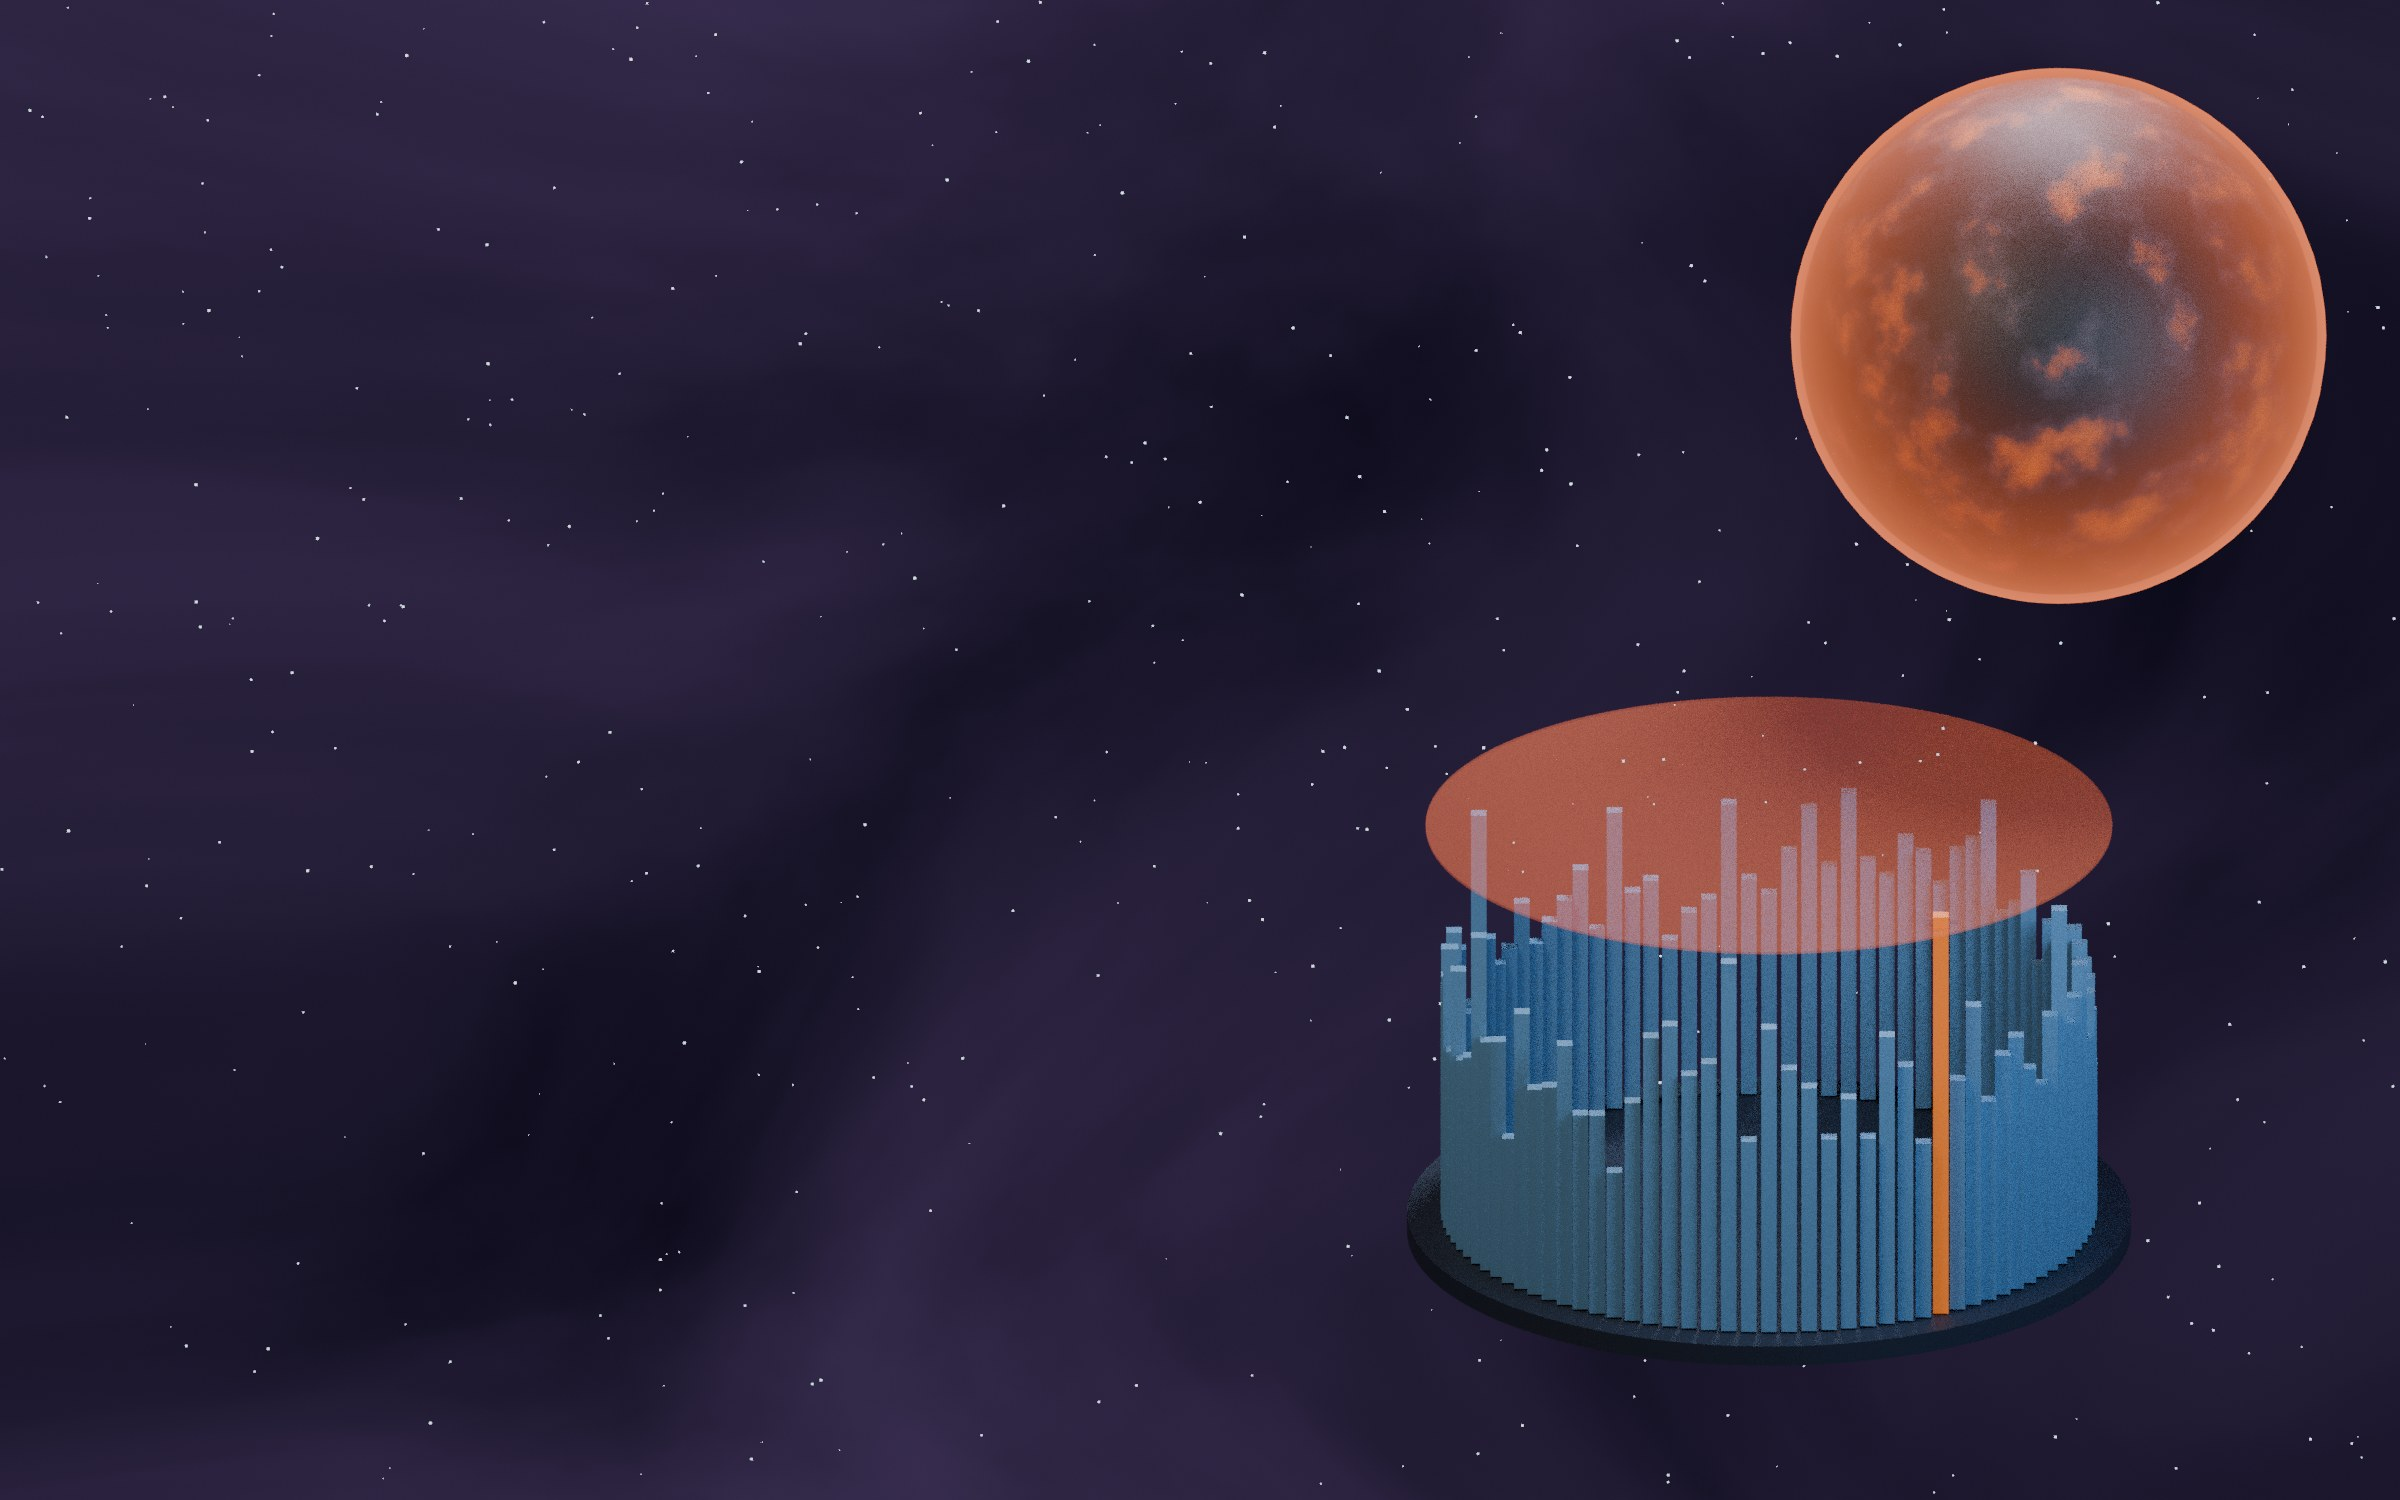
\includegraphics[width=20cm,height=12.5cm]{Scena/copertina.jpg}};}{}
\node[anchor=north west,inner sep=0] at([xshift=1.05cm,yshift=-1.10cm]current page.north west){\color{Mint}\bfseries\fontsize{23}{28}\selectfont SPEDIZIONE P09};
\node[anchor=north west,inner sep=0] at([xshift=1.07cm,yshift=-2.16cm]current page.north west){\color{white}\fontsize{9}{12}\selectfont MACROPROGETTO P09 · SCIENZE DELLA TERRA};
\draw[Mint,line width=1.5pt]([xshift=1.07cm,yshift=-2.78cm]current page.north west)--([xshift=2.6cm,yshift=-2.78cm]current page.north west);
\node[anchor=north west,inner sep=0] at([xshift=1.05cm,yshift=-3.35cm]current page.north west){\begin{minipage}{9.2cm}\raggedright\color{white}\bfseries\fontsize{28.5}{34.5}\selectfont Un livello raro\\e la sua\\incertezza\end{minipage}};
\node[anchor=north west,inner sep=0] at([xshift=1.07cm,yshift=-7.88cm]current page.north west){\begin{minipage}{8.9cm}\raggedright\color{Lilac}\fontsize{12.2}{17}\selectfont Cento massimi annuali di portata\end{minipage}};
\node[anchor=north west,inner sep=0] at([xshift=1.07cm,yshift=-8.70cm]current page.north west){\begin{minipage}{8.9cm}\raggedright\color{white!75}\fontsize{10.3}{14.5}\selectfont Massimi annuali, distribuzione di Gumbel e rischio su un orizzonte temporale\end{minipage}};
\node[anchor=north west,inner sep=0] at([xshift=1.07cm,yshift=-10.52cm]current page.north west){\color{white}\fontsize{10.5}{14}\selectfont GeoStat Lab · corso di Marzio De Corato};
\node[anchor=north west,inner sep=0] at([xshift=1.07cm,yshift=-11.17cm]current page.north west){\color{Mint}\fontsize{8.8}{11}\selectfont\href{https://creativecommons.org/licenses/by-nc-sa/4.0/}{Impaginazione da Tessera · CC BY-NC-SA 4.0}};
\end{tikzpicture}\end{frame}

\begin{frame}[plain]\hypertarget{slide2}{}
\bookmark[level=1,page=2]{Indice della presentazione}
\begin{tikzpicture}[remember picture,overlay]
\PilotChrome{Indice della presentazione}{PERCORSO}{2}{I titoli dell’indice aprono i capitoli. Il nome del capitolo in alto riporta a questa pagina.}
\node[anchor=north west,inner sep=0] at([xshift=.96cm,yshift=-2.12cm]current page.north west){\Colonna{9.40cm}{\PLabel{Capitoli}
{\fontsize{10.7}{13.5}\selectfont\hyperlink{slide4}{Unità annuale e distribuzione dei massimi\hfill 4}\par}\vspace{.16cm}
{\fontsize{10.7}{13.5}\selectfont\hyperlink{slide7}{Stima di Gumbel e livello di ritorno\hfill 7}\par}\vspace{.16cm}
{\fontsize{10.7}{13.5}\selectfont\hyperlink{slide12}{Ricampionamento e incertezza condizionata\hfill 12}\par}\vspace{.16cm}
{\fontsize{10.7}{13.5}\selectfont\hyperlink{slide15}{Rischio temporale e sensibilità della coda\hfill 15}\par}\vspace{.16cm}
{\fontsize{10.7}{13.5}\selectfont\hyperlink{slide18}{Laboratori della spedizione\hfill 18}\par}\vspace{.16cm}

}};
\node[anchor=north west,inner sep=0] at([xshift=10.85cm,yshift=-2.12cm]current page.north west){\Colonna{8.16cm}{\PLabel{Percorso di lettura}
\PBody{Il percorso definisce l’unità annuale, stima il modello di Gumbel e il livello di ritorno, ricampiona l’intero stimatore e traduce la probabilità annua in un rischio su più anni. I laboratori finali riprendono le tre fasi della spedizione.}
\PInfo{Le pagine Scenario A e Confronto riprendono gli esperimenti nel browser con dati sintetici. I valori di partenza del simulatore differiscono da quelli del caso.}
\href{https://marzione00.github.io/Lab_Geo/\#modulo-P09}{\color{Classical}\bfseries Apri la spedizione P09 su GeoStat Lab}
}};
\end{tikzpicture}\end{frame}

\begin{frame}[plain]\hypertarget{slide3}{}
\bookmark[level=1,page=3]{Quale portata ha probabilità annua di superamento dell’uno per cento, e con quale incertezza?}
\begin{tikzpicture}[remember picture,overlay]
\PilotChrome{{\fontsize{15.3}{19}\selectfont Quale portata ha probabilità annua di superamento dell’uno per cento, e con quale incertezza?}}{IL CASO GUIDA}{3}{La copertina è una scena illustrativa: le colonne riproducono i cento massimi, il disco il livello centennale stimato.}
\node[anchor=north west,inner sep=0] at([xshift=.96cm,yshift=-2.12cm]current page.north west){\Colonna{9.40cm}{{\centering\resizebox{0.97\linewidth}{!}{\begin{tikzpicture}[x=1cm,y=1cm,every node/.style={font=\sffamily\fontsize{10}{12}\selectfont,text=Ink}]
\draw[draw=Classical,fill=Classical!8,rounded corners=2mm,line width=.7pt] (0,0.00) rectangle (8.6,-0.78);
\node[circle,anchor=center,fill=Classical,inner sep=0,minimum size=.5cm,text=white,font=\sffamily\bfseries\fontsize{9}{10}\selectfont] at (.48,-0.39) {1};
\node[anchor=west,text width=7.4cm,align=left] at (.95,-0.39) {Unità annuale e distribuzione dei massimi};
\draw[pEdge] (.48,-0.80)--(.48,-1.02);
\draw[draw=Classical,fill=Classical!8,rounded corners=2mm,line width=.7pt] (0,-1.04) rectangle (8.6,-1.82);
\node[circle,anchor=center,fill=Classical,inner sep=0,minimum size=.5cm,text=white,font=\sffamily\bfseries\fontsize{9}{10}\selectfont] at (.48,-1.43) {2};
\node[anchor=west,text width=7.4cm,align=left] at (.95,-1.43) {Stima di Gumbel e livello di ritorno};
\draw[pEdge] (.48,-1.84)--(.48,-2.06);
\draw[draw=Classical,fill=Classical!8,rounded corners=2mm,line width=.7pt] (0,-2.08) rectangle (8.6,-2.86);
\node[circle,anchor=center,fill=Classical,inner sep=0,minimum size=.5cm,text=white,font=\sffamily\bfseries\fontsize{9}{10}\selectfont] at (.48,-2.47) {3};
\node[anchor=west,text width=7.4cm,align=left] at (.95,-2.47) {Ricampionamento e incertezza condizionata};
\draw[pEdge] (.48,-2.88)--(.48,-3.10);
\draw[draw=Classical,fill=Classical!8,rounded corners=2mm,line width=.7pt] (0,-3.12) rectangle (8.6,-3.90);
\node[circle,anchor=center,fill=Classical,inner sep=0,minimum size=.5cm,text=white,font=\sffamily\bfseries\fontsize{9}{10}\selectfont] at (.48,-3.51) {4};
\node[anchor=west,text width=7.4cm,align=left] at (.95,-3.51) {Rischio temporale e sensibilità della coda};
\draw[pEdge] (.48,-3.92)--(.48,-4.14);
\draw[draw=GeoB,fill=GeoB!8,rounded corners=2mm,line width=.7pt] (0,-4.16) rectangle (8.6,-4.94);
\node[circle,anchor=center,fill=GeoB,inner sep=0,minimum size=.5cm,text=white,font=\sffamily\bfseries\fontsize{9}{10}\selectfont] at (.48,-4.55) {L};
\node[anchor=west,text width=7.4cm,align=left] at (.95,-4.55) {Laboratori della spedizione};
\end{tikzpicture}
}\par}
\PSmall{Capitoli della spedizione; L indica i laboratori conclusivi.}
}};
\node[anchor=north west,inner sep=0] at([xshift=10.85cm,yshift=-2.12cm]current page.north west){\Colonna{8.16cm}{\PLabel{Il caso}
\PBody{Cento massimi annuali di portata, simulati per gli anni dal 1920 al 2019, alimentano una stima del livello centennale con il modello di Gumbel. Il ricampionamento e la forma della coda misurano due fonti di incertezza diverse.}
\PInfo{Seguiremo il livello dalla stima dei momenti al bootstrap, poi la probabilità di superamento su un orizzonte di più anni.}
}};
\end{tikzpicture}\end{frame}

\begin{frame}[plain]\hypertarget{slide4}{}
\bookmark[level=0,page=4]{Unità annuale e distribuzione dei massimi}
\bookmark[level=1,page=4]{Il bersaglio è un quantile dei massimi annuali}
\begin{tikzpicture}[remember picture,overlay]
\PilotChrome{Il bersaglio è un quantile dei massimi annuali}{UNITÀ ANNUALE E DISTRIBUZIONE DEI MASSIMI}{4}{La probabilità del livello di ritorno si riferisce alla distribuzione della variabile massima annuale.}
\node[anchor=north west,inner sep=0] at([xshift=.96cm,yshift=-2.12cm]current page.north west){\Colonna{9.40cm}{{\centering\resizebox{0.90\linewidth}{!}{\begin{tikzpicture}[x=1cm,y=-.87cm,every node/.style={font=\fontsize{12.2}{15}\selectfont,text=Ink},arr/.style={-{Stealth[length=2mm]},line width=.8pt,draw=Classical}]\path[use as bounding box] (0,0) rectangle (7.45,6.2);
\draw[draw=Classical,fill=Classical!8,rounded corners=2pt,line width=.7pt] (0.6,0.8) rectangle (6.8,2.1);
\node[anchor=center,text=Ink,font=\fontsize{13}{15}\selectfont,text width=5.8cm,align=center] at (3.7,1.45) {Portate entro ogni anno};
\draw[arr,draw=Classical] (3.7,2.4)--(3.7,3.1);
\draw[draw=Quantum,fill=Quantum!8,rounded corners=2pt,line width=.7pt] (1.3,3.4) rectangle (6.1,4.7);
\node[anchor=center,text=Ink,font=\fontsize{15}{15}\selectfont] at (3.7,4.05) {$M_y=\max_{t\in y}Q_t$};
\node[anchor=center,text=Ink,font=\fontsize{11.5}{15}\selectfont,text width=6.8cm,align=center] at (3.7,5.8) {Una riga rappresenta un massimo annuale.};

\end{tikzpicture}}\par}
\PSmall{$Q_t$: portata al tempo t; $M_y$: massimo nell’anno y. La tabella contiene un solo valore per anno, in m³/s.}
}};
\node[anchor=north west,inner sep=0] at([xshift=10.85cm,yshift=-2.12cm]current page.north west){\Colonna{8.16cm}{\PBody{Il progetto utilizza cento massimi annuali di portata, simulati per gli anni dal 1920 al 2019, per stimare un livello con probabilità annua di superamento pari all’uno per cento. L’unità della tabella è l’anno, del quale viene conservato il solo massimo. Il procedimento collega controllo della serie, adattamento di Gumbel, livello di ritorno e ricampionamento. La natura sintetica dei dati consente di esercitare il calcolo, mentre qualsiasi applicazione a un bacino reale richiederebbe un esame della copertura e della storia idrologica.}
}};
\end{tikzpicture}\end{frame}

\begin{frame}[plain]\hypertarget{slide5}{}
\bookmark[level=1,page=5]{La completezza precede la scelta distributiva}
\begin{tikzpicture}[remember picture,overlay]
\PilotChrome{La completezza precede la scelta distributiva}{UNITÀ ANNUALE E DISTRIBUZIONE DEI MASSIMI}{5}{Una sequenza annuale senza righe mancanti non dimostra, da sola, copertura completa delle osservazioni originarie.}
\node[anchor=north west,inner sep=0] at([xshift=.96cm,yshift=-2.12cm]current page.north west){\Colonna{9.40cm}{{\centering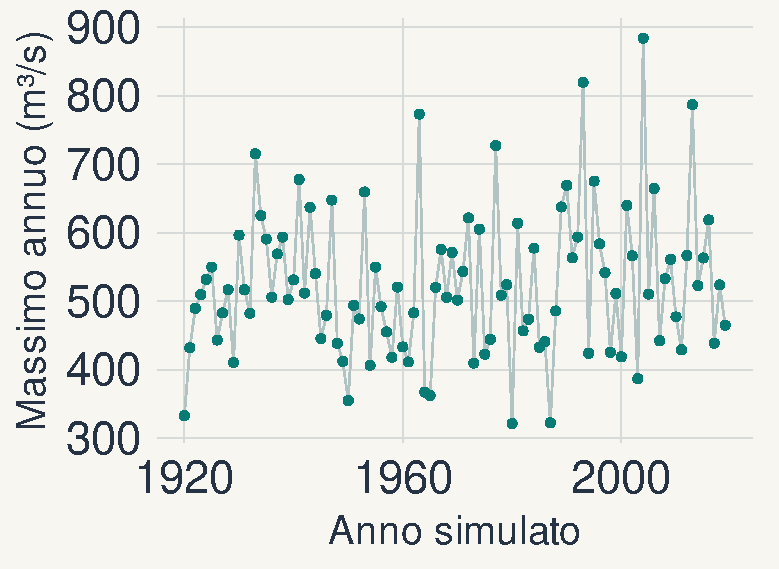
\includegraphics[width=\linewidth,height=6.15cm,keepaspectratio]{Figure/F01.pdf}\par}
\PSmall{Cento massimi annuali sintetici, espressi in metri cubi al secondo.}
}};
\node[anchor=north west,inner sep=0] at([xshift=10.85cm,yshift=-2.12cm]current page.north west){\Colonna{8.16cm}{\PBody{L’audit verifica anni unici e consecutivi, portate finite e positive e presenza di cento osservazioni. Questi controlli garantiscono la coerenza della tabella fornita, senza ricostruire la completezza delle misure giornaliere che avrebbero generato un archivio reale. Un massimo calcolato su pochi giorni potrebbe infatti sottostimare quello dell’anno completo. Analogamente, modifiche strumentali, regolazione del bacino o cambiamenti climatici potrebbero compromettere l’interpretazione di tutti gli anni come realizzazioni della stessa distribuzione.}
}};
\end{tikzpicture}\end{frame}

\begin{frame}[plain]\hypertarget{slide6}{}
\bookmark[level=1,page=6]{Il rango costruisce un riferimento empirico}
\begin{tikzpicture}[remember picture,overlay]
\PilotChrome{Il rango costruisce un riferimento empirico}{UNITÀ ANNUALE E DISTRIBUZIONE DEI MASSIMI}{6}{Una posizione grafica del rango è una convenzione descrittiva, non una frequenza nota senza errore.}
\node[anchor=north west,inner sep=0] at([xshift=.96cm,yshift=-2.12cm]current page.north west){\Colonna{9.40cm}{{\centering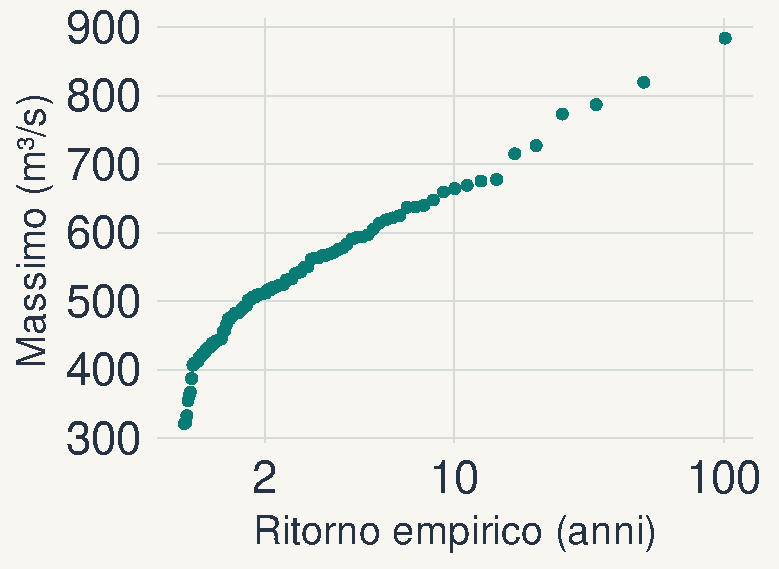
\includegraphics[width=\linewidth,height=6.15cm,keepaspectratio]{Figure/F02.pdf}\par}
\PSmall{n = 100 anni; r = 1 per il massimo, 100 per il minimo. p: superamento empirico; T: ritorno in anni, su scala logaritmica.}
}};
\node[anchor=north west,inner sep=0] at([xshift=10.85cm,yshift=-2.12cm]current page.north west){\Colonna{8.16cm}{\PBody{Ordinando i massimi dal maggiore al minore, il rango viene trasformato in una probabilità empirica di superamento attraverso il denominatore cento più uno. Il suo reciproco definisce una posizione grafica del tempo di ritorno, secondo una convenzione dichiarata. Al valore più elevato viene così associato un ritorno empirico di 101 anni. Questa assegnazione facilita il confronto con un modello continuo, ma rimane incerta soprattutto nella coda, dove ogni punto dipende da pochissime osservazioni.}
\par\smallskip{\centering\adjustbox{max width=.98\linewidth}{$\displaystyle \widehat p_r=\frac{r}{n+1},\qquad \widehat T_r=\frac{n+1}{r}$}\par\smallskip}
}};
\end{tikzpicture}\end{frame}

\begin{frame}[plain]\hypertarget{slide7}{}
\bookmark[level=0,page=7]{Stima di Gumbel e livello di ritorno}
\bookmark[level=1,page=7]{Gumbel descrive posizione e scala della coda}
\begin{tikzpicture}[remember picture,overlay]
\PilotChrome{Gumbel descrive posizione e scala della coda}{STIMA DI GUMBEL E LIVELLO DI RITORNO}{7}{Il livello raro dipende dalla forma della coda specificata nel modello dei massimi.}
\node[anchor=north west,inner sep=0] at([xshift=.96cm,yshift=-2.12cm]current page.north west){\Colonna{9.40cm}{{\centering\resizebox{0.90\linewidth}{!}{\begin{tikzpicture}[x=1cm,y=-.87cm,every node/.style={font=\fontsize{12.2}{15}\selectfont,text=Ink},arr/.style={-{Stealth[length=2mm]},line width=.8pt,draw=Classical}]\path[use as bounding box] (0,0) rectangle (7.45,6.2);
\node[anchor=center,text=Ink,font=\fontsize{12}{15}\selectfont,text width=6.8cm,align=center] at (3.7,0.6) {La soglia divide due probabilità};
\draw[draw=Classical,fill=Classical!8,rounded corners=2pt,line width=.7pt] (0.7,2) rectangle (5.8,3.2);
\draw[draw=Quantum,fill=Quantum!8,rounded corners=2pt,line width=.7pt] (5.8,2) rectangle (6.8,3.2);
\node[anchor=center,text=Ink,font=\fontsize{16}{15}\selectfont] at (3.1,2.6) {$F(q)$};
\node[anchor=center,text=Ink,font=\fontsize{12}{15}\selectfont,text width=2cm,align=center] at (6.3,4.1) {$1-F(q)$};
\draw[Quantum,line width=.8pt] (5.8,1.5)--(5.8,3.6);
\node[anchor=center,text=Ink,font=\fontsize{15}{15}\selectfont] at (5.8,1.1) {$q$};
\node[anchor=center,text=Ink,font=\fontsize{10.8}{15}\selectfont,text width=6.8cm,align=center] at (3.7,5.7) {Schema delle probabilità, senza proporzione di scala.};

\end{tikzpicture}}\par}
\PSmall{$F(q)=P(M\leq q)$, con M massimo annuale; q: soglia; a: posizione; b: scala positiva. q, a e b sono in m³/s.}
}};
\node[anchor=north west,inner sep=0] at([xshift=10.85cm,yshift=-2.12cm]current page.north west){\Colonna{8.16cm}{\PBody{La distribuzione di Gumbel rappresenta i massimi attraverso un parametro di posizione e una scala positiva. Il parametro di scala governa la dispersione e la crescita dei quantili elevati, mentre la posizione trasla la distribuzione nella misura della portata. La scelta corrisponde a una specificazione della coda, che dovrà essere discussa insieme a stazionarietà e indipendenza annuale. L’adattamento del progetto assume quindi una famiglia probabilistica precisa e non ricava la sua validità dalla sola possibilità di stimarne i parametri.}
\par\smallskip{\centering\adjustbox{max width=.98\linewidth}{$\displaystyle F(q)=\exp\!\left[-\exp\!\left(-\frac{q-a}{b}\right)\right],\qquad b>0$}\par\smallskip}
}};
\end{tikzpicture}\end{frame}

\begin{frame}[plain]\hypertarget{slide8}{}
\bookmark[level=1,page=8]{I momenti collegano dati e parametri}
\begin{tikzpicture}[remember picture,overlay]
\PilotChrome{I momenti collegano dati e parametri}{STIMA DI GUMBEL E LIVELLO DI RITORNO}{8}{La formula dello stimatore e la convenzione della varianza devono accompagnare i parametri riportati.}
\node[anchor=north west,inner sep=0] at([xshift=.96cm,yshift=-2.12cm]current page.north west){\Colonna{9.40cm}{\PBody{Il progetto stima la scala moltiplicando la deviazione standard campionaria per la radice di sei e dividendo per pi greco. La posizione si ottiene sottraendo dalla media il prodotto fra tale scala e la costante di Eulero. La deviazione standard di R usa il denominatore n meno uno, convenzione finita qui esplicitata. Si ottengono posizione circa 476,262 e scala circa 82,961 metri cubi al secondo; entrambi i parametri conservano dunque l’unità della portata.}
\par\smallskip{\centering\adjustbox{max width=.98\linewidth}{$\displaystyle \begin{gathered}\widehat b=s\frac{\sqrt6}{\pi},\qquad\widehat a=\overline M-\gamma\widehat b\\\gamma\simeq0{,}577215665\end{gathered}$}\par\smallskip}
}};
\node[anchor=north west,inner sep=0] at([xshift=10.85cm,yshift=-2.12cm]current page.north west){\Colonna{8.16cm}{\PInfo{$\bar M$: media dei cento massimi; s: deviazione standard con denominatore 99; $\gamma$: costante di Eulero–Mascheroni. Le relazioni teoriche sono $E(M)=a+\gamma b$ e $\operatorname{Var}(M)=\pi^2b^2/6$. Sostituire i momenti campionari definisce lo stimatore dichiarato, che può differire dalla massima verosimiglianza.}
}};
\end{tikzpicture}\end{frame}

\begin{frame}[plain]\hypertarget{slide9}{}
\bookmark[level=1,page=9]{L’inversione della distribuzione verifica il calcolo}
\begin{tikzpicture}[remember picture,overlay]
\PilotChrome{{\fontsize{15.3}{19}\selectfont L’inversione della distribuzione verifica il calcolo}}{STIMA DI GUMBEL E LIVELLO DI RITORNO}{9}{Un’identità numerica verifica l’implementazione; la validità della famiglia probabilistica richiede evidenze ulteriori.}
\node[anchor=north west,inner sep=0] at([xshift=.96cm,yshift=-2.12cm]current page.north west){\Colonna{9.40cm}{\PBody{Il quantile di probabilità p si ottiene invertendo la funzione cumulativa mediante due logaritmi. Per un ritorno di cento anni si utilizza p uguale a 0,99, ottenendo circa 857,895 metri cubi al secondo. Il controllo numerico reinserisce il quantile nella distribuzione e verifica che la probabilità recuperata coincida con quella richiesta. La prova controlla la coerenza delle funzioni e della formula, lasciando alla diagnosi statistica e all’analisi idrologica la valutazione delle ipotesi del modello.}
\par\smallskip{\centering\adjustbox{max width=.98\linewidth}{$\displaystyle q_T=\widehat a-\widehat b\log[-\log(1-1/T)]$}\par\smallskip}
\PSmall{$T>1$: ritorno in anni; $p=1-1/T$: probabilità cumulativa. $\hat a=476,262$ e $\hat b=82,961$ m³/s; log è naturale.}
}};
\node[anchor=north west,inner sep=0] at([xshift=10.85cm,yshift=-2.12cm]current page.north west){\Colonna{8.16cm}{\begin{tcolorbox}[enhanced,arc=1.7mm,boxrule=.6pt,colback=white,colframe=Classical!60!Navy,colbacktitle=Navy,coltitle=white,fonttitle=\bfseries\small,title={R · calcolo riproducibile},left=1.7mm,right=1.3mm,top=1.1mm,bottom=1.1mm,before skip=1mm,after skip=1.0mm]\lstinputlisting[style=GeoR,language=R,basicstyle=\ttfamily\fontsize{8.6}{11.4}\selectfont]{Codice/livello.R}\end{tcolorbox}
\PLabel{Risultato in R}
\begin{tcolorbox}[colback=GeoTint,colframe=Rule,boxrule=.5pt,arc=1.4mm,left=2mm,right=1mm,top=1mm,bottom=1mm]{\fontsize{8.4}{10.9}\selectfont\ttfamily \mbox{\ \ \ \ \ \ \ \ a\ \ \ \ \ \ \ \ \ b\ \ \ \ \ \ q100\ \ \ \ \ \ q500\ }\\\mbox{476.26161\ \ 82.96115\ 857.89528\ 991.74961\ }}\end{tcolorbox}
}};
\end{tikzpicture}\end{frame}

\begin{frame}[plain]\hypertarget{slide10}{}
\bookmark[level=1,page=10]{Il confronto dei quantili esamina l’adattamento}
\begin{tikzpicture}[remember picture,overlay]
\PilotChrome{Il confronto dei quantili esamina l’adattamento}{STIMA DI GUMBEL E LIVELLO DI RITORNO}{10}{La diagnosi della coda deve essere interpretata rispetto al numero effettivo di osservazioni estreme.}
\node[anchor=north west,inner sep=0] at([xshift=.96cm,yshift=-2.12cm]current page.north west){\Colonna{9.40cm}{{\centering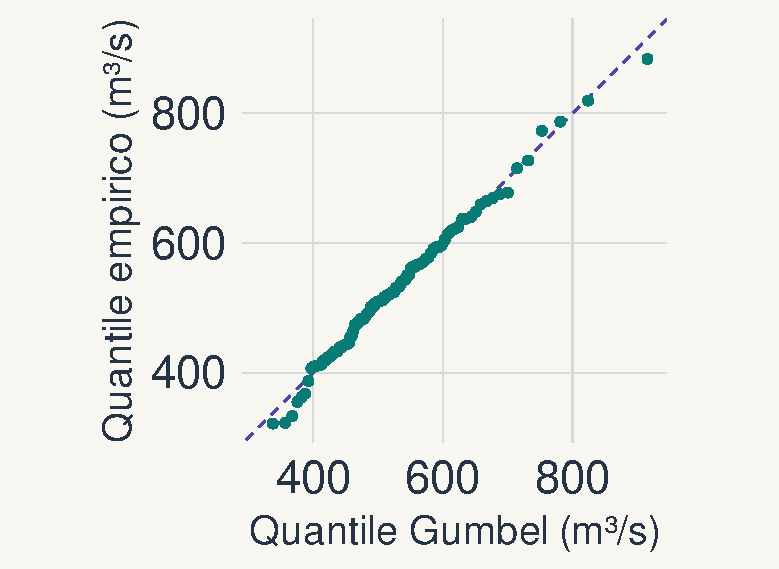
\includegraphics[width=\linewidth,height=6.15cm,keepaspectratio]{Figure/F03.pdf}\par}
\PSmall{Quantili di Gumbel e osservati; riferimento: bisettrice.}
}};
\node[anchor=north west,inner sep=0] at([xshift=10.85cm,yshift=-2.12cm]current page.north west){\Colonna{8.16cm}{\PBody{Il diagramma confronta quantili empirici e quantili di Gumbel calcolati alle stesse posizioni probabilistiche. La bisettrice rappresenta concordanza, mentre scostamenti sistematici nella parte superiore suggerirebbero differenze nella coda. Entrambi gli assi adottano la stessa scala e l’unità della portata. Con cento osservazioni, l’assenza di una deviazione evidente non garantisce una descrizione accurata di probabilità molto piccole: i livelli rari dipendono proprio dalla regione in cui il sostegno empirico è più limitato.}
}};
\end{tikzpicture}\end{frame}

\begin{frame}[plain]\hypertarget{slide11}{}
\bookmark[level=1,page=11]{L’estrapolazione cresce con il tempo di ritorno}
\begin{tikzpicture}[remember picture,overlay]
\PilotChrome{L’estrapolazione cresce con il tempo di ritorno}{STIMA DI GUMBEL E LIVELLO DI RITORNO}{11}{La distanza fra orizzonte raro e lunghezza del record rende più rilevante la sensibilità del modello di coda.}
\node[anchor=north west,inner sep=0] at([xshift=.96cm,yshift=-2.12cm]current page.north west){\Colonna{9.40cm}{{\centering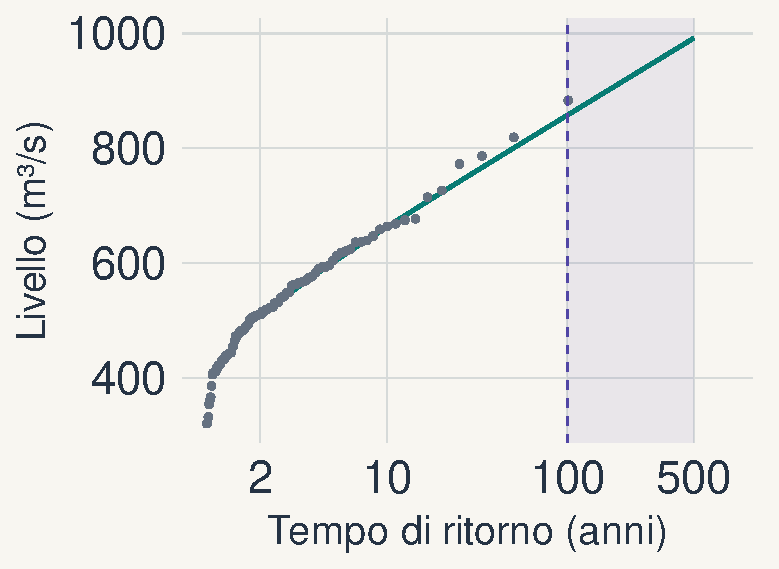
\includegraphics[width=\linewidth,height=6.15cm,keepaspectratio]{Figure/F04.pdf}\par}
\PSmall{Livelli stimati e ranghi empirici; evidenziati ritorni oltre cento anni.}
}};
\node[anchor=north west,inner sep=0] at([xshift=10.85cm,yshift=-2.12cm]current page.north west){\Colonna{8.16cm}{\PBody{La curva dei livelli cresce lungo un asse logaritmico del tempo di ritorno. A cinquecento anni il valore stimato è circa 991,750 metri cubi al secondo, superiore al massimo osservato di circa 883,687. L’area evidenziata segnala tempi di ritorno maggiori della lunghezza centennale della serie, rendendo visibile il ruolo crescente del modello nella coda. La lunghezza del record orienta la discussione sul sostegno empirico e sulla sensibilità alle ipotesi distributive, senza costituire una soglia matematica di validità.}
}};
\end{tikzpicture}\end{frame}

\begin{frame}[plain]\hypertarget{slide12}{}
\bookmark[level=0,page=12]{Ricampionamento e incertezza condizionata}
\bookmark[level=1,page=12]{Ogni replica ricostruisce l’intero stimatore}
\begin{tikzpicture}[remember picture,overlay]
\PilotChrome{Ogni replica ricostruisce l’intero stimatore}{RICAMPIONAMENTO E INCERTEZZA CONDIZIONATA}{12}{La replica deve ripetere tutte le operazioni con cui il campione determina la stima finale.}
\node[anchor=north west,inner sep=0] at([xshift=.96cm,yshift=-2.12cm]current page.north west){\Colonna{9.40cm}{{\centering\resizebox{0.90\linewidth}{!}{\begin{tikzpicture}[x=1cm,y=-.87cm,every node/.style={font=\fontsize{12.2}{15}\selectfont,text=Ink},arr/.style={-{Stealth[length=2mm]},line width=.8pt,draw=Classical}]\path[use as bounding box] (0,0) rectangle (7.45,6.2);
\draw[draw=Classical,fill=Classical!8,rounded corners=2pt,line width=.7pt] (0.6,0.5) rectangle (6.8,1.8);
\node[anchor=center,text=Ink,font=\fontsize{12}{15}\selectfont,text width=5.9cm,align=center] at (3.7,1.15) {Cento anni estratti con reinserimento};
\draw[arr,draw=Classical] (3.7,2.1)--(3.7,2.7);
\draw[draw=Classical,fill=Classical!8,rounded corners=2pt,line width=.7pt] (0.6,3) rectangle (3.3,4.3);
\node[anchor=center,text=Ink,font=\fontsize{15}{15}\selectfont] at (1.95,3.65) {$\overline M^*,\ s^*$};
\draw[draw=Quantum,fill=Quantum!8,rounded corners=2pt,line width=.7pt] (4,3) rectangle (6.8,4.3);
\node[anchor=center,text=Ink,font=\fontsize{15}{15}\selectfont] at (5.4,3.65) {$\widehat a^*,\ \widehat b^*$};
\draw[arr,draw=Classical] (3.4,3.65)--(3.9,3.65);
\node[anchor=center,text=Ink,font=\fontsize{14}{15}\selectfont,text width=6.8cm,align=center] at (3.7,5.6) {$q_{100}^{*}=Q(0{,}99;\widehat a^*,\widehat b^*)$};

\end{tikzpicture}}\par}
\PSmall{L’asterisco indica la replica: $\bar M^*$ e $s^*$ sono media e deviazione; $\hat a^*,\hat b^*$ i parametri; $q_{100}^*$ il livello a cento anni.}
}};
\node[anchor=north west,inner sep=0] at([xshift=10.85cm,yshift=-2.12cm]current page.north west){\Colonna{8.16cm}{\PBody{Il bootstrap estrae con reinserimento cento massimi annuali e ricalcola media, deviazione standard, parametri di Gumbel e livello centennale. Ripetendo l’intera sequenza, la variabilità dei momenti si propaga fino alla quantità finale. Il piano conserva 1999 vettori di indici, così da poter ricostruire ogni replica. Il ricampionamento annuale presuppone unità scambiabili e rappresenta la variabilità campionaria entro la famiglia adottata; dipendenza temporale o evoluzione della distribuzione richiederebbero uno schema coerente con tali strutture.}
}};
\end{tikzpicture}\end{frame}

\begin{frame}[plain]\hypertarget{slide13}{}
\bookmark[level=1,page=13]{L’intervallo percentile mantiene le sue condizioni}
\begin{tikzpicture}[remember picture,overlay]
\PilotChrome{L’intervallo percentile mantiene le sue condizioni}{RICAMPIONAMENTO E INCERTEZZA CONDIZIONATA}{13}{Un intervallo bootstrap va associato allo stimatore, all’unità ricampionata e alle fonti di incertezza effettivamente rappresentate.}
\node[anchor=north west,inner sep=0] at([xshift=.96cm,yshift=-2.12cm]current page.north west){\Colonna{9.40cm}{\PBody{I quantili 2,5\% e 97,5\% delle 1999 stime sono circa 789,160 e 923,105 metri cubi al secondo. L’intervallo percentile riassume la dispersione della stima centennale nel riferimento ricampionato. La sua ampiezza non incorpora automaticamente errori strumentali, mancata copertura annuale, cambiamenti del regime o scelta della famiglia di coda. Il frammento legge il piano conservato e ricostruisce i quantili, consentendo di confrontare il risultato con quello prodotto dallo script completo senza generare nuove estrazioni.}
}};
\node[anchor=north west,inner sep=0] at([xshift=10.85cm,yshift=-2.12cm]current page.north west){\Colonna{8.16cm}{\begin{tcolorbox}[enhanced,arc=1.7mm,boxrule=.6pt,colback=white,colframe=Classical!60!Navy,colbacktitle=Navy,coltitle=white,fonttitle=\bfseries\small,title={R · calcolo riproducibile},left=1.7mm,right=1.3mm,top=1.1mm,bottom=1.1mm,before skip=1mm,after skip=1.0mm]\lstinputlisting[style=GeoR,language=R,basicstyle=\ttfamily\fontsize{8.6}{11.4}\selectfont]{Codice/bootstrap.R}\end{tcolorbox}
\PLabel{Risultato in R}
\begin{tcolorbox}[colback=GeoTint,colframe=Rule,boxrule=.5pt,arc=1.4mm,left=2mm,right=1mm,top=1mm,bottom=1mm]{\fontsize{8.4}{10.9}\selectfont\ttfamily \mbox{\ \ \ \ 2.5\%\ \ \ \ \ \ 50\%\ \ \ \ 97.5\%\ }\\\mbox{789.1598\ 853.9918\ 923.1048\ }}\end{tcolorbox}
}};
\end{tikzpicture}\end{frame}

\begin{frame}[plain]\hypertarget{slide14}{}
\bookmark[level=1,page=14]{La distribuzione ricampionata conserva l’asimmetria}
\begin{tikzpicture}[remember picture,overlay]
\PilotChrome{{\fontsize{15.3}{19}\selectfont La distribuzione ricampionata conserva l’asimmetria}}{RICAMPIONAMENTO E INCERTEZZA CONDIZIONATA}{14}{La distribuzione di uno stimatore e quella di una futura osservazione hanno oggetti e scale interpretative differenti.}
\node[anchor=north west,inner sep=0] at([xshift=.96cm,yshift=-2.12cm]current page.north west){\Colonna{9.40cm}{{\centering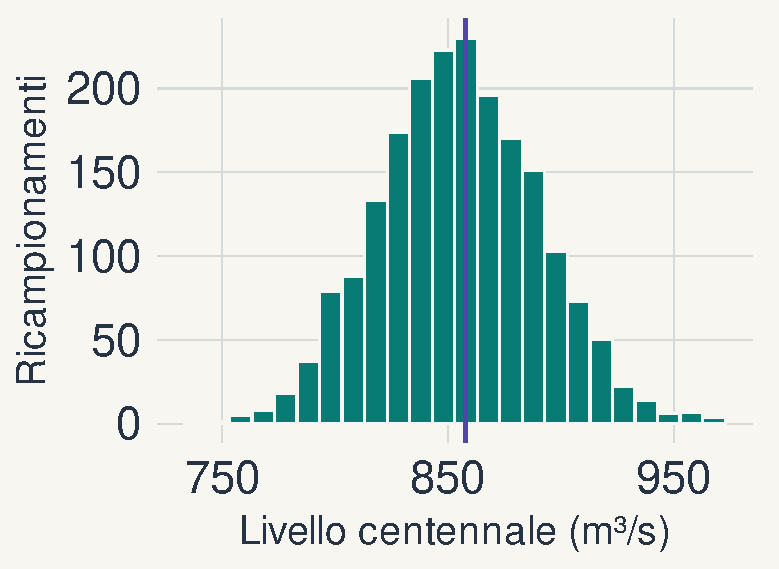
\includegraphics[width=\linewidth,height=6.15cm,keepaspectratio]{Figure/F05.pdf}\par}
\PSmall{1999 stime bootstrap del livello centennale; stima originale in viola.}
}};
\node[anchor=north west,inner sep=0] at([xshift=10.85cm,yshift=-2.12cm]current page.north west){\Colonna{8.16cm}{\PBody{L’istogramma mostra le stime del livello centennale ottenute dai campioni ricostruiti, mentre la linea viola indica la stima sul campione originale. La distribuzione permette di valutare forma e dispersione senza ridurre il risultato ai soli estremi dell’intervallo. Le repliche che estraggono più volte i massimi maggiori possono modificare sia la media sia la scala, producendo un effetto sul quantile raro. La figura rappresenta incertezza dello stimatore e deve essere distinta dalla distribuzione delle future portate massime.}
}};
\end{tikzpicture}\end{frame}

\begin{frame}[plain]\hypertarget{slide15}{}
\bookmark[level=0,page=15]{Rischio temporale e sensibilità della coda}
\bookmark[level=1,page=15]{Cento anni di ritorno non fissano una scadenza}
\begin{tikzpicture}[remember picture,overlay]
\PilotChrome{Cento anni di ritorno non fissano una scadenza}{RISCHIO TEMPORALE E SENSIBILITÀ DELLA CODA}{15}{Il tempo di ritorno è una trasformazione di probabilità, la cui interpretazione sull’orizzonte richiede ipotesi temporali.}
\node[anchor=north west,inner sep=0] at([xshift=.96cm,yshift=-2.12cm]current page.north west){\Colonna{9.40cm}{{\centering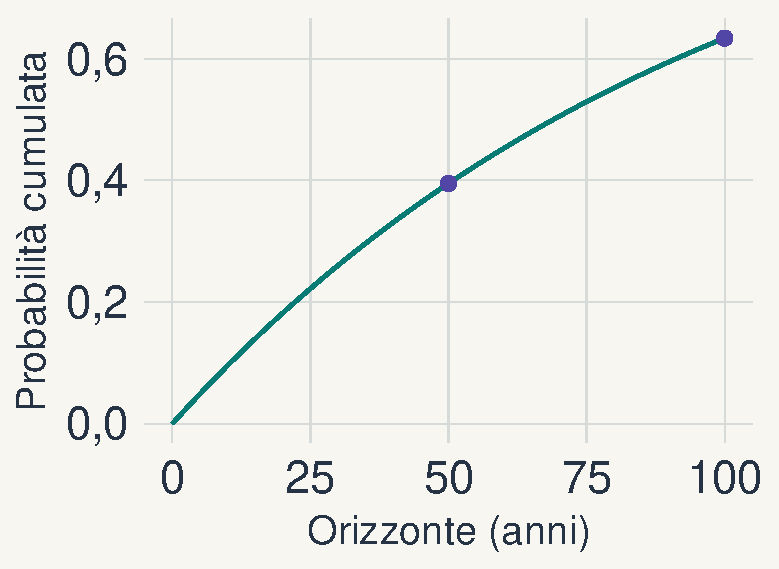
\includegraphics[width=\linewidth,height=6.15cm,keepaspectratio]{Figure/F06.pdf}\par}
\PSmall{$M_y$: massimo dell’anno y; $q_T$: livello con superamento annuo 1/T; h: orizzonte in anni. Curva per T = 100.}
}};
\node[anchor=north west,inner sep=0] at([xshift=10.85cm,yshift=-2.12cm]current page.north west){\Colonna{8.16cm}{\PBody{Un tempo di ritorno di cento anni corrisponde, nel modello stazionario, a una probabilità annua di superamento pari a un centesimo. Assumendo anche l’indipendenza fra anni, la probabilità di almeno un superamento in h anni si ottiene dal complemento dell’assenza di superamenti. Essa vale circa 39,5\% in cinquant’anni e 63,4\% in cento. Il livello centennale può pertanto essere superato in anni consecutivi, mentre un intero secolo potrebbe trascorrere senza superamenti.}
\par\smallskip{\centering\adjustbox{max width=.98\linewidth}{$\displaystyle P\!\left(\max_{1\le y\le h}M_y>q_T\right)=1-\left(1-\frac1T\right)^h$}\par\smallskip}
}};
\end{tikzpicture}\end{frame}

\begin{frame}[plain]\hypertarget{slide16}{}
\bookmark[level=1,page=16]{La forma della coda modifica i livelli più rari}
\begin{tikzpicture}[remember picture,overlay]
\PilotChrome{La forma della coda modifica i livelli più rari}{RISCHIO TEMPORALE E SENSIBILITÀ DELLA CODA}{16}{La sensibilità strutturale della coda va discussa separatamente dall’incertezza campionaria entro una famiglia.}
\node[anchor=north west,inner sep=0] at([xshift=.96cm,yshift=-2.12cm]current page.north west){\Colonna{9.40cm}{{\centering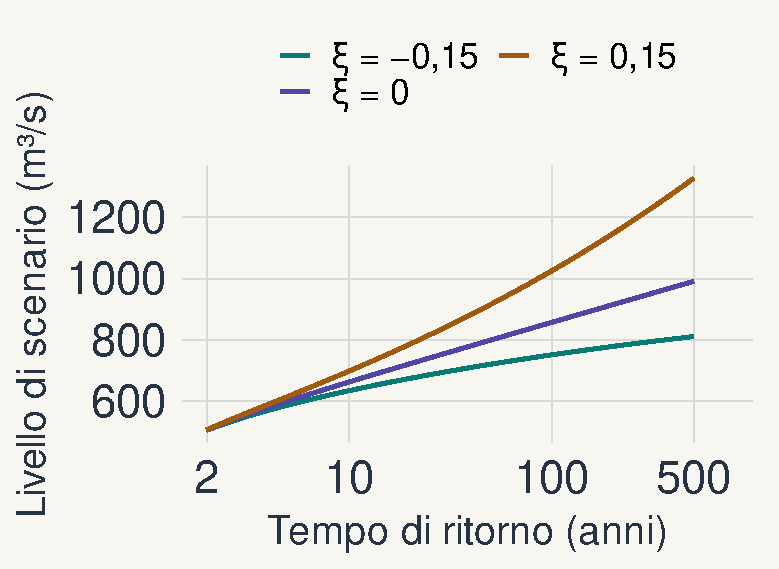
\includegraphics[width=\linewidth,height=6.15cm,keepaspectratio]{Figure/F07.pdf}\par}
\PSmall{a = 476,262, b = 82,961 m³/s; $p=1-1/T$, 0 < p < 1; $\xi$: forma. Per $\xi=0$ si usa il limite Gumbel.}
}};
\node[anchor=north west,inner sep=0] at([xshift=10.85cm,yshift=-2.12cm]current page.north west){\Colonna{8.16cm}{\PBody{La sensibilità confronta tre distribuzioni GEV con forma meno 0,15, zero e più 0,15, mantenendo posizione e scala ai valori stimati per Gumbel. La forma nulla coincide con il modello precedente; gli altri due casi rappresentano scenari dichiarati, distinti da adattamenti alternativi ai dati. La divergenza cresce verso i tempi di ritorno maggiori, mostrando quanto un quantile remoto dipenda dalla struttura della coda. La figura completa il bootstrap, poiché esamina una fonte di variazione che il ricampionamento entro Gumbel mantiene fissa.}
\par\smallskip{\centering\adjustbox{max width=.98\linewidth}{$\displaystyle Q_\xi(p)=a+\frac b\xi\{[-\log p]^{-\xi}-1\},\qquad\xi\ne0$}\par\smallskip}
}};
\end{tikzpicture}\end{frame}

\begin{frame}[plain]\hypertarget{slide17}{}
\bookmark[level=1,page=17]{Consegna: giustificare il livello e il suo uso}
\begin{tikzpicture}[remember picture,overlay]
\PilotChrome{Consegna: giustificare il livello e il suo uso}{RISCHIO TEMPORALE E SENSIBILITÀ DELLA CODA}{17}{Il significato applicativo del livello raro dipende dal collegamento fra dati, probabilità annuale e orizzonte decisionale.}
\node[anchor=north west,inner sep=0] at([xshift=.96cm,yshift=-2.12cm]current page.north west){\Colonna{9.40cm}{\PBody{La relazione presenta audit annuale, stima dei parametri, confronto dei quantili, livelli di ritorno, distribuzione bootstrap e rischio sull’orizzonte. L’esercizio richiede di ricavare il livello centennale dalla probabilità di superamento e di calcolare il rischio su cinquant’anni. Una seconda discussione distingue gli effetti del ricampionamento da quelli della forma GEV. La conclusione riporta stima e intervallo insieme alle ipotesi di stazionarietà, indipendenza e famiglia di coda, conservando la natura sintetica dell’archivio.}
}};
\node[anchor=north west,inner sep=0] at([xshift=10.85cm,yshift=-2.12cm]current page.north west){\Colonna{8.16cm}{\PInfo{R/P09\_figure.R integra le attività sui massimi, sui momenti di Gumbel, sui livelli e sul bootstrap sviluppate in M14. Sono conservati tutti i piani delle 1999 repliche, le stime e le curve di sensibilità. L’esercizio fornisce una base metodologica, senza dimensionare opere o formulare una valutazione di rischio per un bacino reale.}
}};
\end{tikzpicture}\end{frame}

\begin{frame}[plain]\hypertarget{slide18}{}
\bookmark[level=0,page=18]{Laboratori della spedizione}
\bookmark[level=1,page=18]{Tre fasi della spedizione nel laboratorio}
\begin{tikzpicture}[remember picture,overlay]
\PilotChrome{Tre fasi della spedizione nel laboratorio}{LABORATORI DELLA SPEDIZIONE}{18}{Gli esperimenti usano dati sintetici; la conclusione sul caso resta quella ottenuta dai cento massimi.}
\node[anchor=north west,inner sep=0] at([xshift=.96cm,yshift=-2.12cm]current page.north west){\Colonna{9.40cm}{{\centering\resizebox{0.97\linewidth}{!}{\begin{tikzpicture}[x=1cm,y=1cm,every node/.style={font=\sffamily\fontsize{9.2}{11}\selectfont,text=Ink}]
\node[draw=Classical,fill=Classical,rounded corners=2mm,text=white,text width=2.45cm,align=flush center,minimum height=1.55cm,anchor=west,font=\sffamily\bfseries\fontsize{9.2}{11}\selectfont] (f0) at (0,0.00) {1. Definire l’evento};
\node[draw=Classical!60,fill=Classical!6,rounded corners=1.5mm,line width=.6pt,text width=2.8cm,align=flush center,minimum height=1.55cm,anchor=west] (e00) at (2.95,0.00) {Dalle osservazioni ai massimi annuali\\[1pt]{\fontsize{7.6}{9}\selectfont\color{Muted}m14-massimi}};
\node[draw=Rule,fill=white,rounded corners=1.5mm,line width=.6pt,text width=2.8cm,align=flush center,minimum height=1.55cm,anchor=west] (e01) at (6.10,0.00) {Superamenti e separazione degli episodi\\[1pt]{\fontsize{7.6}{9}\selectfont\color{Muted}m14-episodi}};
\draw[pEdge] (f0.east)--(e00.west);
\node[draw=Classical,fill=Classical,rounded corners=2mm,text=white,text width=2.45cm,align=flush center,minimum height=1.55cm,anchor=west,font=\sffamily\bfseries\fontsize{9.2}{11}\selectfont] (f1) at (0,-1.95) {2. Stimare e ricampionare};
\draw[pEdge] (f0.south)--(f1.north);
\node[draw=Classical!60,fill=Classical!6,rounded corners=1.5mm,line width=.6pt,text width=2.8cm,align=flush center,minimum height=1.55cm,anchor=west] (e10) at (2.95,-1.95) {Adattamento di Gumbel ai massimi\\[1pt]{\fontsize{7.6}{9}\selectfont\color{Muted}m14-gumbel}};
\node[draw=Rule,fill=white,rounded corners=1.5mm,line width=.6pt,text width=2.8cm,align=flush center,minimum height=1.55cm,anchor=west] (e11) at (6.10,-1.95) {Livelli di ritorno e incertezza bootstrap\\[1pt]{\fontsize{7.6}{9}\selectfont\color{Muted}m14-livelli-rari}};
\draw[pEdge] (f1.east)--(e10.west);
\node[draw=Classical,fill=Classical,rounded corners=2mm,text=white,text width=2.45cm,align=flush center,minimum height=1.55cm,anchor=west,font=\sffamily\bfseries\fontsize{9.2}{11}\selectfont] (f2) at (0,-3.90) {3. Interpretare il rischio};
\draw[pEdge] (f1.south)--(f2.north);
\node[draw=Classical!60,fill=Classical!6,rounded corners=1.5mm,line width=.6pt,text width=2.8cm,align=flush center,minimum height=1.55cm,anchor=west] (e20) at (2.95,-3.90) {Sensibilità alla forma della coda GEV\\[1pt]{\fontsize{7.6}{9}\selectfont\color{Muted}m14-gev}};
\node[draw=Rule,fill=white,rounded corners=1.5mm,line width=.6pt,text width=2.8cm,align=flush center,minimum height=1.55cm,anchor=west] (e21) at (6.10,-3.90) {Tempo di ritorno e orizzonte temporale\\[1pt]{\fontsize{7.6}{9}\selectfont\color{Muted}m14-ritorno}};
\draw[pEdge] (f2.east)--(e20.west);
\end{tikzpicture}
}\par}
\PSmall{Fasi della spedizione. Il primo esperimento di ogni fase ha le pagine Scenario A e Confronto.}
}};
\node[anchor=north west,inner sep=0] at([xshift=10.85cm,yshift=-2.12cm]current page.north west){\Colonna{8.16cm}{\PBody{Gli esperimenti della lezione Ignis ripetono su dati sintetici tre passaggi della spedizione: definire l’evento estremo, stimare il modello di coda, interpretare il rischio.}
\vspace{.2cm}\PLabel{Altri esperimenti delle fasi}
\PLab{https://marzione00.github.io/Lab_Geo/\#laboratorio/m14-episodi}{Superamenti e separazione degli episodi · m14-episodi}
\PLab{https://marzione00.github.io/Lab_Geo/\#laboratorio/m14-livelli-rari}{Livelli di ritorno e incertezza bootstrap · m14-livelli-rari}
\PLab{https://marzione00.github.io/Lab_Geo/\#laboratorio/m14-ritorno}{Tempo di ritorno e orizzonte temporale · m14-ritorno}
\PLab{https://marzione00.github.io/Lab_Geo/\#laboratorio/m14-conseguenze}{Pericolosità e conseguenze · m14-conseguenze}
}};
\end{tikzpicture}\end{frame}

\begin{frame}[plain]\hypertarget{slide19}{}
\bookmark[level=1,page=19]{Dalle osservazioni ai massimi annuali}
\begin{tikzpicture}[remember picture,overlay]
\PilotChrome{Dalle osservazioni ai massimi annuali}{LABORATORI DELLA SPEDIZIONE}{19}{Esaminare la distribuzione dei massimi di blocchi indipendenti.}
\node[anchor=north west,inner sep=0] at([xshift=.96cm,yshift=-2.12cm]current page.north west){\Colonna{9.40cm}{{\centering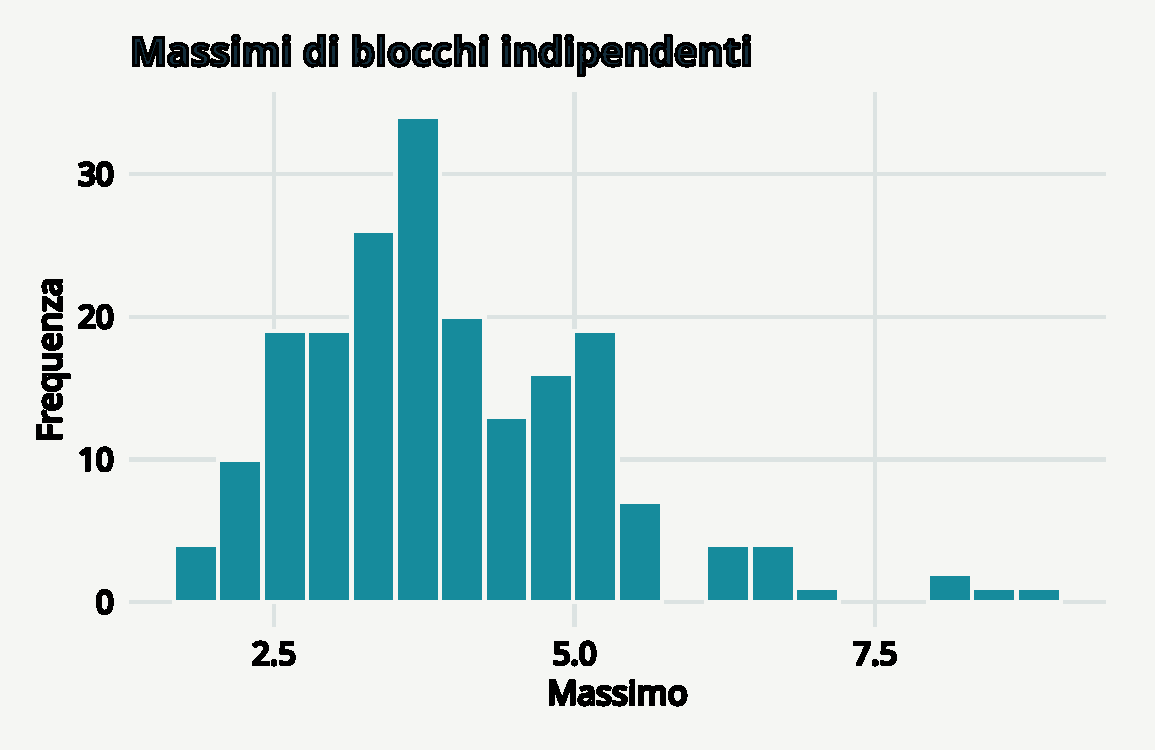
\includegraphics[width=\linewidth,height=6.0cm,keepaspectratio]{Esperimenti/m14-massimi-A.pdf}\par}
\PSmall{Osservazioni per blocco: 30. Seme: 17.}
}};
\node[anchor=north west,inner sep=0] at([xshift=10.85cm,yshift=-2.12cm]current page.north west){\Colonna{8.16cm}{\PLabel{Scenario A · simulazione}
\PBody{Il massimo di un blocco dipende sia dalla distribuzione delle singole osservazioni sia dal numero di occasioni nelle quali possono comparire valori elevati. L’esperimento genera osservazioni esponenziali indipendenti con tasso unitario, raggruppandole in blocchi della dimensione scelta. Per ciascuna replica conserva soltanto il massimo, del quale mostra la distribuzione empirica.}
\par\smallskip{\centering\adjustbox{max width=.98\linewidth}{$\displaystyle P(M_m\le x)=F(x)^m$}\par\smallskip}
\PSmall{$M_m$ è il massimo di m osservazioni indipendenti con la stessa funzione di distribuzione F. La probabilità che il massimo non superi x coincide con la probabilità che tutte le osservazioni non lo superino.}
}};
\node[anchor=north east,inner sep=0] at([xshift=17.1cm,yshift=-12.04cm]current page.north west){\fontsize{7.7}{9}\selectfont \href{https://marzione00.github.io/Lab_Geo/\#laboratorio/m14-massimi}{\color{Classical}\bfseries Apri il laboratorio · m14-massimi}};
\end{tikzpicture}\end{frame}

\begin{frame}[plain]\hypertarget{slide20}{}
\bookmark[level=1,page=20]{Confronto | Dalle osservazioni ai massimi annuali}
\begin{tikzpicture}[remember picture,overlay]
\PilotChrome{Confronto | Dalle osservazioni ai massimi annuali}{LABORATORI DELLA SPEDIZIONE}{20}{Il massimo cresce con il numero di opportunità di osservare valori elevati.}
\node[anchor=north west,inner sep=0] at([xshift=.96cm,yshift=-2.12cm]current page.north west){\Colonna{9.40cm}{{\centering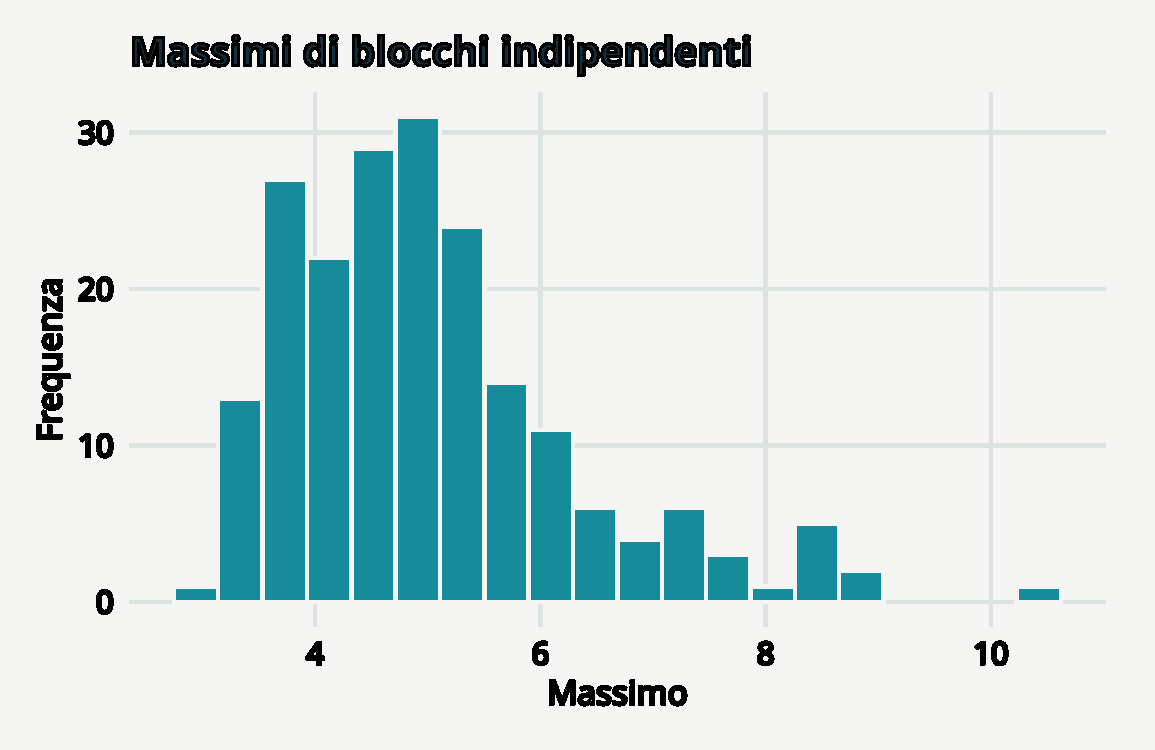
\includegraphics[width=\linewidth,height=5.6cm,keepaspectratio]{Esperimenti/m14-massimi-B.pdf}\par}
\PSmall{Osservazioni per blocco: 30 $\to$ 90. Tutti gli altri parametri e il seme sono fissi.}
}};
\node[anchor=north west,inner sep=0] at([xshift=10.85cm,yshift=-2.12cm]current page.north west){\Colonna{8.16cm}{\PLabel{Confronto fra gli scenari}
{\fontsize{10.2}{12.8}\selectfont\begin{tabular}{@{}>{\raggedright\arraybackslash}p{0.48\linewidth}@{\hspace{.13cm}}>{\raggedright\arraybackslash}p{0.224\linewidth}@{\hspace{.13cm}}>{\raggedright\arraybackslash}p{0.224\linewidth}@{}}\toprule Grandezza & A & B\\[2.3pt]
\midrule 
Media dei massimi & 3,96 & 5,03\\[2.3pt]
Quantile teorico 95\% & 6,37 & 7,47\\[2.3pt]
Quantile empirico 95\% & 6,14 & 7,58\\[2.3pt]
\bottomrule\end{tabular}\par}
\vspace{.25cm}\PBody{Un blocco di 90 osservazioni offre più occasioni per un estremo. La distribuzione di origine è la stessa, mentre la media dei massimi cresce.}
}};
\node[anchor=north east,inner sep=0] at([xshift=17.1cm,yshift=-12.04cm]current page.north west){\fontsize{7.7}{9}\selectfont \href{https://marzione00.github.io/Lab_Geo/\#laboratorio/m14-massimi}{\color{Classical}\bfseries Apri il laboratorio · m14-massimi}};
\end{tikzpicture}\end{frame}

\begin{frame}[plain]\hypertarget{slide21}{}
\bookmark[level=1,page=21]{Adattamento di Gumbel ai massimi}
\begin{tikzpicture}[remember picture,overlay]
\PilotChrome{Adattamento di Gumbel ai massimi}{LABORATORI DELLA SPEDIZIONE}{21}{Confrontare distribuzione empirica e modello stimato ai momenti.}
\node[anchor=north west,inner sep=0] at([xshift=.96cm,yshift=-2.12cm]current page.north west){\Colonna{9.40cm}{{\centering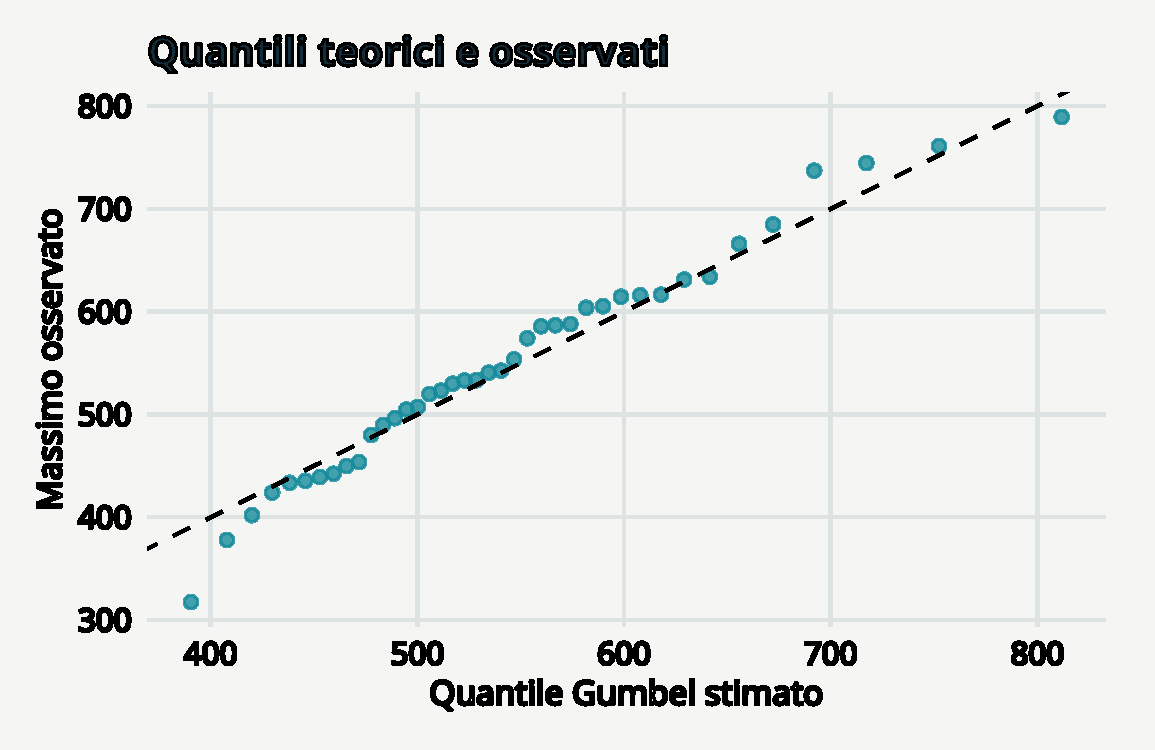
\includegraphics[width=\linewidth,height=6.0cm,keepaspectratio]{Esperimenti/m14-gumbel-A.pdf}\par}
\PSmall{Anni osservati: 40. Seme: 17.}
}};
\node[anchor=north west,inner sep=0] at([xshift=10.85cm,yshift=-2.12cm]current page.north west){\Colonna{8.16cm}{\PLabel{Scenario A · simulazione}
\PBody{La distribuzione Gumbel per massimi descrive una famiglia asimmetrica caratterizzata da posizione e scala positiva. Il programma genera un record sintetico da parametri fissati e li ristima mediante media e deviazione standard campionarie. Il controllo sulla lunghezza del record permette di osservare quanto le stime dipendano dall’informazione disponibile.}
\par\smallskip{\centering\adjustbox{max width=.98\linewidth}{$\displaystyle F(x)=\exp\{-\exp[-(x-\mu)/\beta]\},\quad\beta>0$}\par\smallskip}
\PSmall{$\mu$ è il parametro di posizione e β la scala, che deve essere positiva. F(x) è la probabilità cumulativa dei massimi. La stima ai momenti utilizza $\hat\beta=s\sqrt{6}/\pi$ e $\hat\mu=\bar x-\gamma\hat\beta$, con γ costante di Eulero–Mascheroni.}
}};
\node[anchor=north east,inner sep=0] at([xshift=17.1cm,yshift=-12.04cm]current page.north west){\fontsize{7.7}{9}\selectfont \href{https://marzione00.github.io/Lab_Geo/\#laboratorio/m14-gumbel}{\color{Classical}\bfseries Apri il laboratorio · m14-gumbel}};
\end{tikzpicture}\end{frame}

\begin{frame}[plain]\hypertarget{slide22}{}
\bookmark[level=1,page=22]{Confronto | Adattamento di Gumbel ai massimi}
\begin{tikzpicture}[remember picture,overlay]
\PilotChrome{Confronto | Adattamento di Gumbel ai massimi}{LABORATORI DELLA SPEDIZIONE}{22}{La verifica dell’adattamento deve accompagnare l’estrapolazione alle code.}
\node[anchor=north west,inner sep=0] at([xshift=.96cm,yshift=-2.12cm]current page.north west){\Colonna{9.40cm}{{\centering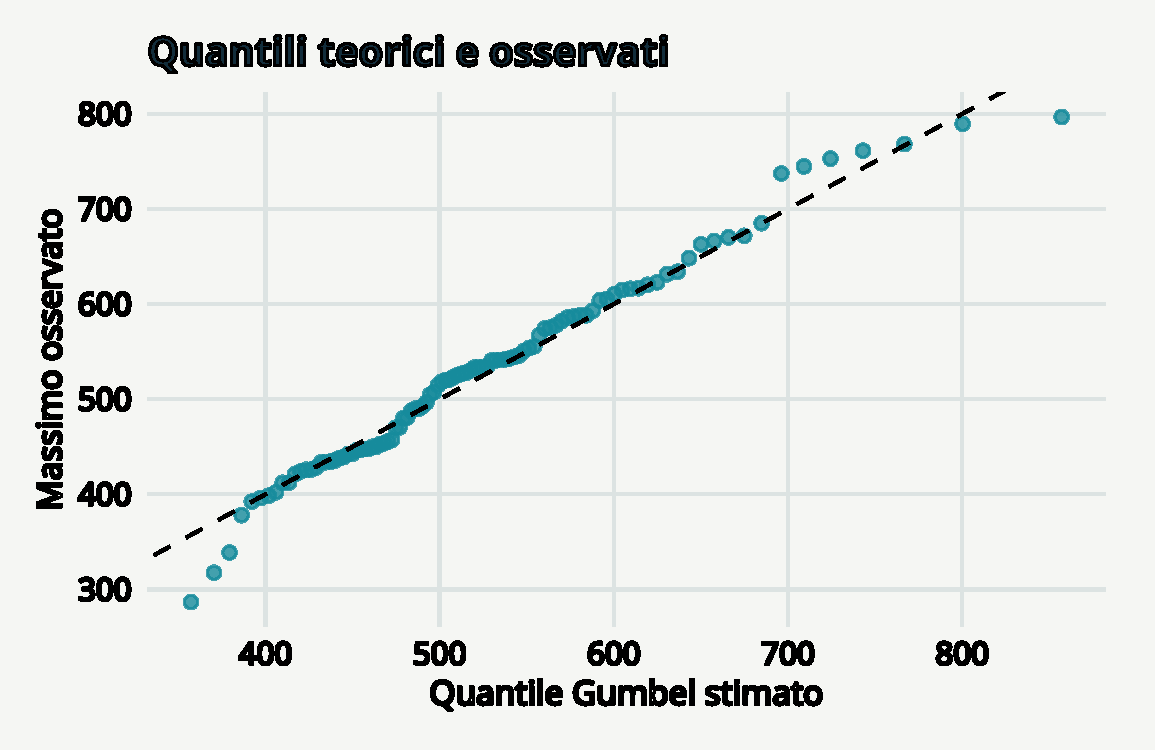
\includegraphics[width=\linewidth,height=5.6cm,keepaspectratio]{Esperimenti/m14-gumbel-B.pdf}\par}
\PSmall{Anni osservati: 40 $\to$ 100. Tutti gli altri parametri e il seme sono fissi.}
}};
\node[anchor=north west,inner sep=0] at([xshift=10.85cm,yshift=-2.12cm]current page.north west){\Colonna{8.16cm}{\PLabel{Confronto fra gli scenari}
{\fontsize{10.2}{12.8}\selectfont\begin{tabular}{@{}>{\raggedright\arraybackslash}p{0.48\linewidth}@{\hspace{.13cm}}>{\raggedright\arraybackslash}p{0.224\linewidth}@{\hspace{.13cm}}>{\raggedright\arraybackslash}p{0.224\linewidth}@{}}\toprule Grandezza & A & B\\[2.3pt]
\midrule 
Posizione stimata & 501 & 482\\[2.3pt]
Scala stimata & 84 & 81,4\\[2.3pt]
Anni osservati & 40 & 100\\[2.3pt]
\bottomrule\end{tabular}\par}
\vspace{.25cm}\PBody{Con 100 anni il modello usa più osservazioni. Le due stime puntuali illustrano una realizzazione per ciascuna lunghezza del record, non una misura generale del bias.}
}};
\node[anchor=north east,inner sep=0] at([xshift=17.1cm,yshift=-12.04cm]current page.north west){\fontsize{7.7}{9}\selectfont \href{https://marzione00.github.io/Lab_Geo/\#laboratorio/m14-gumbel}{\color{Classical}\bfseries Apri il laboratorio · m14-gumbel}};
\end{tikzpicture}\end{frame}

\begin{frame}[plain]\hypertarget{slide23}{}
\bookmark[level=1,page=23]{Sensibilità alla forma della coda GEV}
\begin{tikzpicture}[remember picture,overlay]
\PilotChrome{Sensibilità alla forma della coda GEV}{LABORATORI DELLA SPEDIZIONE}{23}{Confrontare livelli rari sotto forme di coda differenti.}
\node[anchor=north west,inner sep=0] at([xshift=.96cm,yshift=-2.12cm]current page.north west){\Colonna{9.40cm}{{\centering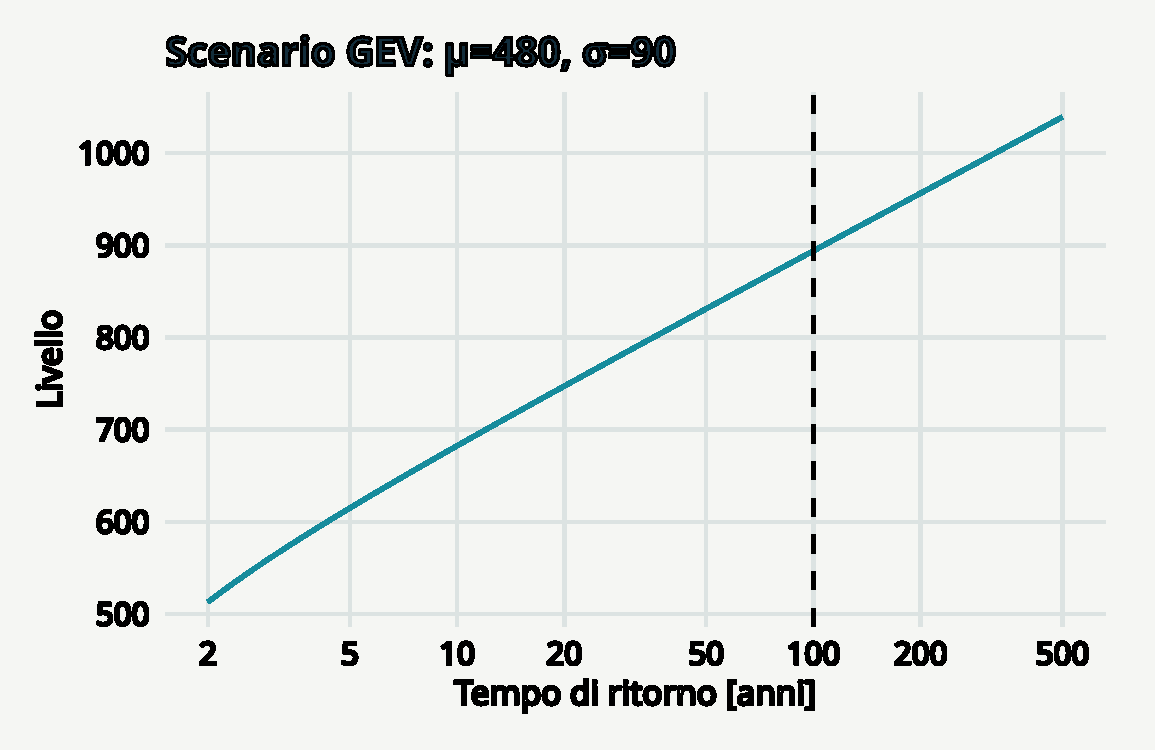
\includegraphics[width=\linewidth,height=6.0cm,keepaspectratio]{Esperimenti/m14-gev-A.pdf}\par}
\PSmall{Parametro di forma $\xi$: 0. Seme: 17.}
}};
\node[anchor=north west,inner sep=0] at([xshift=10.85cm,yshift=-2.12cm]current page.north west){\Colonna{8.16cm}{\PLabel{Scenario A · simulazione}
\PBody{La famiglia generalizzata dei valori estremi introduce un parametro di forma che governa il comportamento della coda. Nell’esperimento, posizione e scala rimangono fissate mentre il controllo modifica la forma, rendendo confrontabili scenari di estrapolazione costruiti sulle medesime grandezze di riferimento. Una linea verticale individua il tempo di ritorno interrogato.}
\par\smallskip{\centering\adjustbox{max width=.98\linewidth}{$\displaystyle q_T=\begin{cases}\mu+\dfrac{\sigma}{\xi}\{[-\log(1-1/T)]^{-\xi}-1\},&\xi\ne0\\\mu-\sigma\log[-\log(1-1/T)],&\xi=0\end{cases}$}\par\smallskip}
\PSmall{$\mu$ è la posizione, $\sigma$ la scala positiva, $\xi$ il parametro di forma e T il tempo di ritorno. Per $\xi<0$ il limite superiore è $\mu-\sigma/\xi$; per $\xi=0$ si usa $q_T=\mu-\sigma\log[-\log(1-1/T)]$.}
}};
\node[anchor=north east,inner sep=0] at([xshift=17.1cm,yshift=-12.04cm]current page.north west){\fontsize{7.7}{9}\selectfont \href{https://marzione00.github.io/Lab_Geo/\#laboratorio/m14-gev}{\color{Classical}\bfseries Apri il laboratorio · m14-gev}};
\end{tikzpicture}\end{frame}

\begin{frame}[plain]\hypertarget{slide24}{}
\bookmark[level=1,page=24]{Confronto | Sensibilità alla forma della coda GEV}
\begin{tikzpicture}[remember picture,overlay]
\PilotChrome{Confronto | Sensibilità alla forma della coda GEV}{LABORATORI DELLA SPEDIZIONE}{24}{Le curve rappresentano scenari di sensibilità e non adattamenti alternativi allo stesso record.}
\node[anchor=north west,inner sep=0] at([xshift=.96cm,yshift=-2.12cm]current page.north west){\Colonna{9.40cm}{{\centering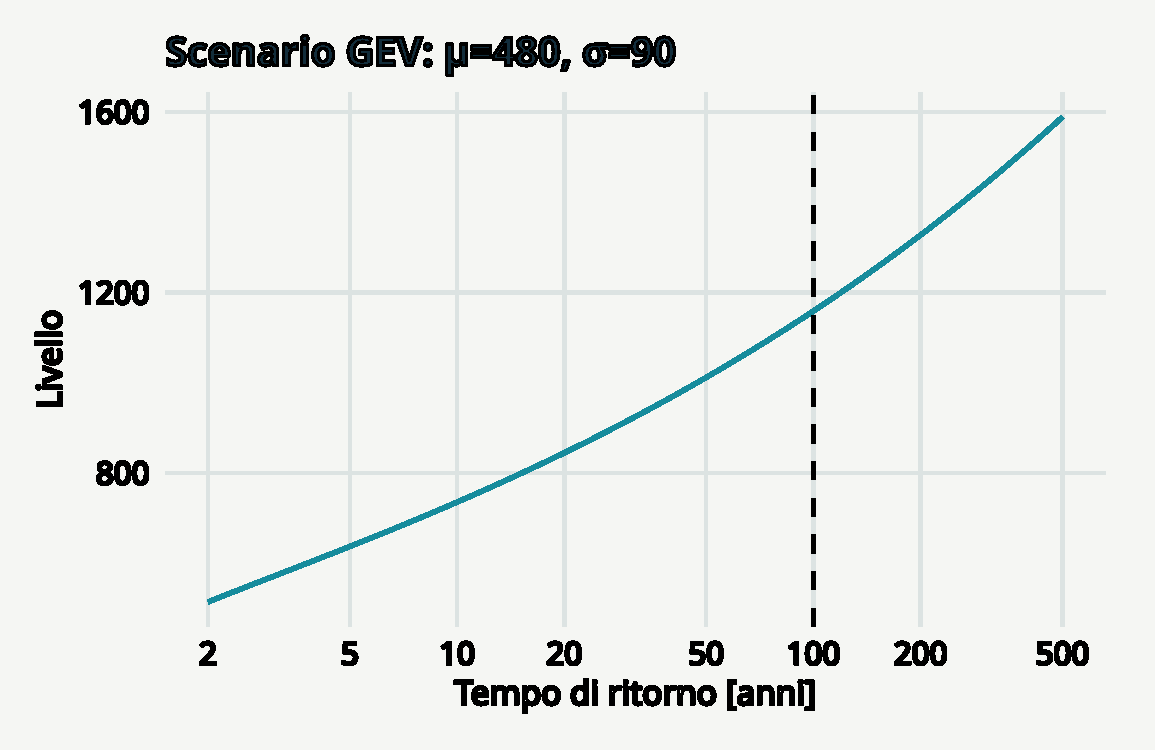
\includegraphics[width=\linewidth,height=5.6cm,keepaspectratio]{Esperimenti/m14-gev-B.pdf}\par}
\PSmall{Parametro di forma $\xi$: 0 $\to$ 0,2. Tutti gli altri parametri e il seme sono fissi.}
}};
\node[anchor=north west,inner sep=0] at([xshift=10.85cm,yshift=-2.12cm]current page.north west){\Colonna{8.16cm}{\PLabel{Confronto fra gli scenari}
{\fontsize{10.2}{12.8}\selectfont\begin{tabular}{@{}>{\raggedright\arraybackslash}p{0.48\linewidth}@{\hspace{.13cm}}>{\raggedright\arraybackslash}p{0.224\linewidth}@{\hspace{.13cm}}>{\raggedright\arraybackslash}p{0.224\linewidth}@{}}\toprule Grandezza & A & B\\[2.3pt]
\midrule 
Livello al T scelto & 894 & 1159\\[2.3pt]
Limite superiore & Non finito & Non finito\\[2.3pt]
Forma $\xi$ & 0 & 0,2\\[2.3pt]
\bottomrule\end{tabular}\par}
\vspace{.25cm}\PBody{Una forma positiva produce una coda più lunga e un livello centennale più alto. Entrambi gli scenari confrontati hanno supporto superiore illimitato.}
}};
\node[anchor=north east,inner sep=0] at([xshift=17.1cm,yshift=-12.04cm]current page.north west){\fontsize{7.7}{9}\selectfont \href{https://marzione00.github.io/Lab_Geo/\#laboratorio/m14-gev}{\color{Classical}\bfseries Apri il laboratorio · m14-gev}};
\end{tikzpicture}\end{frame}

\begin{frame}[plain]\hypertarget{slide25}{}
\bookmark[level=1,page=25]{Dal risultato alla relazione}
\begin{tikzpicture}[remember picture,overlay]
\PilotChrome{Dal risultato alla relazione}{SINTESI}{25}{Riporta livello, unità, tempo di ritorno, intervallo e orizzonte, con le ipotesi sulla coda.}
\node[anchor=north west,inner sep=0] at([xshift=.96cm,yshift=-2.12cm]current page.north west){\Colonna{9.40cm}{\PLabel{Domanda di partenza}
\PBody{Quale portata ha probabilità annua di superamento dell’uno per cento, e con quale incertezza?}
\PLabel{Risultato da discutere}
\PBody{Il modello di Gumbel stima il livello centennale a circa 857,9 m³/s; il bootstrap con 1999 repliche dà un intervallo percentile da circa 789,2 a 923,1 m³/s. La probabilità di almeno un superamento in 50 anni indipendenti è circa 0,395.}
}};
\node[anchor=north west,inner sep=0] at([xshift=10.85cm,yshift=-2.12cm]current page.north west){\Colonna{8.16cm}{\PLabel{Limiti della conclusione}
\PBody{I dati sono sintetici e il calcolo assume indipendenza e stazionarietà fra anni. Con forma della coda pari a −0,15 o +0,15 il livello con tempo di ritorno di 500 anni passa da 991,7 a 811,6 o 1327,8 m³/s.}
\vspace{.4cm}\href{https://marzione00.github.io/Lab_Geo/\#modulo-P10}{\color{Classical}\bfseries Prosegui · P10 · Un’analisi ricostruibile e verificabile}
}};
\end{tikzpicture}\end{frame}

\begin{frame}[plain]\hypertarget{slide26}{}
\bookmark[level=1,page=26]{Fonti, dati e codice per riprodurre le figure}
\begin{tikzpicture}[remember picture,overlay]
\PilotChrome{Fonti, dati e codice per riprodurre le figure}{RIFERIMENTI}{26}{I risultati numerici si riferiscono ai dati e alle ipotesi dichiarate nel caso.}
\node[anchor=north west,inner sep=0] at([xshift=.96cm,yshift=-2.12cm]current page.north west){\Colonna{9.40cm}{\PLabel{Dati e attribuzioni}
\PBody{Dati sintetici del corso (estremi\_v3.csv): cento massimi annuali di portata in metri cubi al secondo, in raccordo con il modulo M14.}
}};
\node[anchor=north west,inner sep=0] at([xshift=10.85cm,yshift=-2.12cm]current page.north west){\Colonna{8.16cm}{\PLabel{Nell’archivio dei sorgenti}
\PBody{Codice contiene i frammenti delle pagine; R contiene lo script P09\_figure.R, che ricostruisce figure e valori dai dati. Esperimenti comprende i programmi dei due scenari, Diagrammi i disegni TikZ modificabili, Scena il modello Blender della copertina.}
\vspace{.4cm}\href{https://marzione00.github.io/Lab_Geo/\#modulo-P09}{\color{Classical}\bfseries Apri la spedizione P09 su GeoStat Lab}
}};
\end{tikzpicture}\end{frame}
\end{document}
